%%%%%%%%%%%%%%%%%%%%%%%%%%%%%%%%%%%%%%%%%%%%%%%%%%%%%%%%%%%%%%%%%%%%%%%%%%%%%%%%
\Chapter{Fundamentals}{}{}
\label{ch:foundations}
\glsresetall
%%%%%%%%%%%%%%%%%%%%%%%%%%%%%%%%%%%%%%%%%%%%%%%%%%%%%%%%%%%%%%%%%%%%%%%%%%%%%%%%
% 
In this chapter, we introduce fundamental terms concerning graph theory
(\cref{ch:foundations:sec:graph-theory}) and graph-theoretical flows
(\cref{ch:foundations:sec:graph-theoretical-flows}). For complexity theory, we
refer to the common literature~\parencite{Gar79,Aus99}. 
% 
The~\acrlong{feas} (\gls{feas}) checks whether for a given supply and demand
there is a feasible (electrical) flow. We give an overview of the different
feasibility problems in power grids
in~\cref{ch:foundations:sec:power-flow-analyses} that form the basis of any
problem in the power grid analysis. We start with
the~\acrlong{ac}~\acrlong{feas} (\gls{ac}~\gls{feas}) and its different
formulations in~\cref{ch:foundations:sec:power-flow-analyses:subsec:AC-Model}.
In the latter section, we define different functions that are used in this
thesis and give a short overview of the common transmission line representations
that are used in the literature. Furthermore, we give an idea of how we are able
to add more complex elements such as transformers and~\acrlong{facts}
(\gls{facts}) to the models without changing the models themselves, but a
component of the analysis.

\gls{ac}~\gls{feas} is~\NP-hard~\parencite{Ver10,Leh16}. Since~\gls{feas} is a
subproblem of all placement problems, we use an approximation
of~\gls{ac}~\gls{feas} that is polynomial time solvable to increase the
(structural) understanding.
In~\cref{ch:foundations:sec:power-flow-analyses:subsec:Lin-DC-Model}, we
introduce different assumptions that result in such a (linear) feasibility
problem commonly known as~\acrlong{dc} (\gls{dc}) \gls{feas}. While the model is
derived from an~\gls{ac} model, we will give the analogies to the~\gls{dc} model
of the~\gls{dc} network to understand the meaning of the name. A feasibility
problem that uses one assumption less than the~\gls{dc} feasibility problem is
denoted by the~\acrlong{sinac}~\gls{feas} (\gls{sinac}), which is described
in~\cref{ch:foundations:sec:power-flow-analyses:subsec:Sin-Model}. The problem
is known to be~\NP-hard~\parencite{Ver10,Bie19}. Afterwards, we discuss the
practicability of the simplifying model assumption
in~\cref{ch:foundations:sec:power-flow-analyses:subsec:AC-vs-DC-Model}.
% 
% At the end
% of this chapter, we give an overview of the experimental setup of the
% simulations of this thesis.
% 
%%%%%%%%%%%%%%%%%%%%%%%%%%%%%%%%%%%%%%%%%%%%%%%%%%%%%%%%%%%%%%%%%%%%%%%%%%%%%%%%
\section{Fundamental Graph-theoretic Terminology}
\label{ch:foundations:sec:graph-theory}
%%%%%%%%%%%%%%%%%%%%%%%%%%%%%%%%%%%%%%%%%%%%%%%%%%%%%%%%%%%%%%%%%%%%%%%%%%%%%%%%  
% 
The underlying power grid is in our case \emph{reciprocal} (also known
as bilateral), \ie, a bidirectional power flow is allowed, and it is common to
give each edge an orientation for notational convenience. Thus, 
the power grid's topological structure can be represented by a
\emph{(simple) undirected graph}~$\glssymbol{graph} =
(\glssymbol{vertices},\glssymbol{undirectededges})$ with a
set~$\glssymbol{vertices}(\glssymbol{graph})$ of \emph{vertices}, representing
buses in our case, and a
set~$\glssymbol{undirectededges}(\glssymbol{graph})\subseteq\binom{\glssymbol{vertices}}{2}$
of~\emph{edges} that is represented by unordered pairs of
vertices~$\undirectededge =
\{\vertexa,\vertexb\}\in\glssymbol{undirectededges}(\glssymbol{graph})$
representing electrical elements such as cables or lines. Note that buses
represent electrical junction points and that an edge can represent devices such
as transformers, circuit breakers, or~\gls{facts}; or simpler elements such as
inductors, resistors, or capacitors. Depending on the literature edges are
sometimes denoted as branches or circuits. The term \emph{simple} denotes that
there is at most one edge per vertex pair allowed.

Even though the underlying power grid is in our case \emph{reciprocal}, it is
common to give each edge an orientation for notational convenience. A
\emph{directed graph} is a tuple~$
  % 
  \glssymbol{graph} 
  = (\glssymbol{vertices},\glssymbol{edges})
  % 
$, where each edge in the set~$\glssymbol{edges}(\glssymbol{graph})$ of edges
has an orientation that is represented by an ordered pair of vertices~$
  % 
  \edge 
  =
  (\vertexa,\vertexb)
  \in
  \glssymbol{edges}(\glssymbol{graph})
  % 
$. If not ambiguous, for~$\glssymbol{vertices}(\glssymbol{graph})$,
$\glssymbol{undirectededges}(\glssymbol{graph})$, and
$\glssymbol{edges}(\glssymbol{graph})$ we simply write~\glssymbol{vertices},
\glssymbol{undirectededges}, and \glssymbol{edges}, respectively.

In general, power grids can have multiple edges between to vertices. There are
multi-graphs~$
  % 
  \glssymbol{graph} 
  = 
  (\glssymbol{vertices},\glssymbol{edges},\paralleledgeMap)
  % 
$ with the multiset~$
  % 
  \glssymbol{edges}
  \subseteq
  \glssymbol{vertices}
  \times
  \glssymbol{vertices}
  % 
$ of edges. Thus, there is a mapping~$
  % 
  \paralleledgeMap
  \colon
  \glssymbol{undirectededges}
  \to
  \{
    \{\vertexa,\vertexb\}
    \mid 
    \vertexa,
    \vertexb
    \in
    \glssymbol{vertices};
    \vertexa
    \not=
    \vertexb
  \}
  % 
$ identifying edges~$
  % 
  \undirectededge_i
  \colon
  \{\vertexa,\vertexb\}^i
  % 
$ with~$1\leq i\leq k$ being the~$k$ parallel edges (\ie, in our case
conductors) that belong to the same electricity link~$\{\vertexa,\vertexb\}$.
Note that in terms of power grids a multi-graph can be easily simplified to a
simple graph
(see~\cref{ch:network-analyzes:sec:reduction-transformation-rules}). Thus, if
not mentioned otherwise, we assume that our graphs are simple and for notational
simplicity use both the directed graph and the underlying undirected graph that
are distinguished by the notation of the edge set.

Vertices that have an edge in common are called \emph{adjacent} and are
\emph{neighbors}. The set of neighbors, \ie, the neighborhood, of a
vertex~\vertexb in an undirected graph is denoted by~$
    % 
    \glssymbol{neighbor}(\vertexb)
    =
    \{
        \vertexa
        \in
        \glssymbol{vertices}
        \mid
        \{\vertexa,\vertexb\}
        \in
        \glssymbol{undirectededges}
    \}
    % 
$. For a vertex~$\vertexb$ in a directed graph, we distinguish between incoming
edges~$(\vertexa,\vertexb)\in\glssymbol{edges}$ and outgoing edges~$
(\vertexb,\vertexc)\in\glssymbol{edges}$ for
all~$\vertexa,\vertexc\in\glssymbol{vertices}$. The neighborhood created by
incoming and outgoing edges is denoted by~$
    % 
    \glssymbol{inneighbor}(\vertexb)
    \coloneqq 
    \{ 
        \vertexa \in \glssymbol{vertices}
        \mid 
        (\vertexa, \vertexb)
        \in
        \glssymbol{edges} 
    \}
    % 
$ and~$
    % 
    \glssymbol{outneighbor}(\vertexb)
    \coloneqq 
    \{ 
        \vertexa \in \glssymbol{vertices}
        \mid 
        (\vertexb, \vertexa)
        \in
        \glssymbol{edges} 
    \}
    % 
$, respectively. A vertex that represents an endpoint of an edge is
\emph{incident} to that very edge. The \emph{degree} of a vertex~\vertexb
denotes the number of edges it is incident to. We distinguish between degree,
in-degree, and out-degree defined
by~$\fmagnitude{\glssymbol{neighbor}(\vertexb)}$,
$\fmagnitude{\glssymbol{inneighbor}(\vertexb)}$,
and~$\fmagnitude{\glssymbol{outneighbor}(\vertexb)}$, respectively.

\textcite[p.13]{Cai12} mention that power grids are planar. A graph is
called~\emph{planar} if it can be embedded into the plane without any edge
crossings, \ie, the edges have no common point, but the two vertices
representing the endpoints of an edge. However, note that there is usually more
than one embedding for a graph~\glssymbol{graph} that is planar. Thus, let us
assume a fixed~\emph{planar embedding}~\glssymbol{embedding} of a
graph~\glssymbol{graph} into the plane
with~$\glssymbol{graph}(\glssymbol{embedding})\cong\glssymbol{graph}$ (\ie,
$\glssymbol{graph}(\glssymbol{embedding})$ is isomorphic to~\glssymbol{graph})
and an injective
function~$\embeddingMap\colon\glssymbol{vertices}\to\reals\times\reals$ meaning
there is a correspondence between the vertices~\glssymbol{vertices} of the graph
and the geometrical points~$\points$ of the plane embedding. An edge
set~$\glssymbol{edges}(\glssymbol{graph})$ of~$\glssymbol{graph}(\embedding)$ is
a subset of a topological space~$\mathcal{T}$, where each edge
in~$\glssymbol{graph}(\embedding)$ is a Jordan curve in~$\mathcal{T}$ and the
incidences and adjacencies are defined accordingly~\parencite{Gro01}.
 
An \emph{induced} subgraph~$\glssymbol{graph} [ \glssymbol{vertices}' ]$ of a
graph~\glssymbol{graph} is a graph~$
    % 
    \subgraph
    =
    (
        \glssymbol{vertices}'
        \subseteq
        \glssymbol{vertices}(\glssymbol{graph}), 
        \{
            (\vertexa,\vertexb)
            \in
            \glssymbol{edges}
            (\glssymbol{graph})
            \mid
            \vertexa,
            \vertexb
            \in
            \glssymbol{vertices}'
        \} 
    )
    % 
$ whose vertices~$\glssymbol{vertices}'$ are a subset of~$\glssymbol{vertices}
(\glssymbol{graph})$ and that has exactly these edges that have both endpoints
in~$\glssymbol{vertices}'$. Note that this definition also applies to undirected
graphs with the set of edges~$\glssymbol{undirectededges}$. Note that a subgraph
that is not induced does not necessarily incorporate all edges, where both
endpoints are in~$\glssymbol{vertices}'$.
 
A \emph{path} from a vertex~\source to a vertex~\sink (or~\source-\sink-path) is
a sequence of edges~$
    % 
    \fpath{}{\source}{\sink} 
    \coloneqq 
    \big( 
        (\source,\vertex_1), 
        (\vertex_1,\vertex_2), 
        \dots,
        (\vertex_{k-1}, \vertex_k), 
        (\vertex_k, \sink) 
    \big)
    % 
$, where two successive edges have an endpoint in common. We call a path
\emph{simple} if no vertex is visited twice and thus, all vertices~$\source,
\vertex_1, \vertex_2,$ $\dots, \vertex_k, \sink$ are distinct. In general, there
is more than one path from~\source to~\sink. We denote the \emph{set of simple
paths} from~\source to~\sink by~$\glssymbol{pathset}(\source,\sink)$. A
\emph{cycle}~$\glssymbol{cycle}$ is a
path~$
    % 
    \fpath{}{\source}{\sink}
    % \in
    % \glssymbol{pathset}(\source,\sink)
    % 
$, where the first and the last vertex are identical meaning~$\source = \sink$.
A cycle is called \emph{simple} if all vertices are distinct with the exception
of~$\source$ and~$\sink$. A graph with no cycles is called \emph{acyclic}.

A \emph{connected component} is a subgraph, where there is a path between each
pair of vertices. Furthermore, we call a graph~\glssymbol{graph}
\emph{connected} if it has one connected component. A \emph{tree} is a connected
graph~$\tree = (\glssymbol{vertices}, \glssymbol{undirectededges})$ that has no
simple cycles. A tree~$\tree$ that connects all vertices of a connected graph~$
    % 
    \glssymbol{graph} 
    = (\glssymbol{vertices},\glssymbol{undirectededges})
    % 
$ is called a \emph{spanning tree} with~$
    % 
    \glssymbol{vertices}(\tree)
    =
    \glssymbol{vertices}(\glssymbol{graph})
    % 
$ and~$
    % 
    \glssymbol{undirectededges}(\tree)
    \subseteq
    \glssymbol{undirectededges}(\glssymbol{graph})
    % 
$ with~$
    % 
    \fmagnitude{\glssymbol{undirectededges}(\tree)} 
    =
    \fmagnitude{\glssymbol{vertices}} 
    - 
    1
    % 
$ being the number of edges. If graph~\glssymbol{graph} is not connected and
has~$k$ connected components then we construct a spanning tree for each
connected component. The set of spanning trees is called spanning forest~\forest
and thus, the number of edges in a spanning forest
is~$
    % 
    \fmagnitude{\glssymbol{vertices}}
    -
    k
    % 
$. Let~\forest be some fixed spanning forest in~\glssymbol{graph}. Edges of
graph~\glssymbol{graph} that are not branches of that spanning forest~\forest
are given by~$
    % 
    \glssymbol{undirectededges}(\glssymbol{graph})
    \setminus
    \glssymbol{undirectededges}(\forest)
    % 
$ and are called \emph{chords} with respect to~\forest. The number of chords is 
given by~$
    % 
    \fmagnitude{\glssymbol{undirectededges}}
    -
    \fmagnitude{\glssymbol{vertices}} 
    +
    k
    % 
$, where~$k$ is the number of connected components.

An \emph{edge cut-set}~$\cutset\subsetneq\glssymbol{undirectededges}$ is a set
of edges with~$\glssymbol{undirectededges}\setminus\cutset$ that decomposes the
graph~\glssymbol{graph} into at least two new components. In terms
of~\textcite{Whi32a} or~\textcite[p.27]{Ses61} this means that the
rank~$\rank(\glssymbol{graph})$ of the graph~\glssymbol{graph} reduces by at
least one. The \emph{rank} of a graph is defined
by~$\fmagnitude{\glssymbol{vertices}} - k$, where~$k$ is the number of connected
components. Note that cycles and cut-sets are closely related to each other as
shown in~\cref{ch:network-analysis}.

A graph can be represented in different ways as a matrix. Note that we represent
a \emph{matrix} with bold capital letters and \emph{vectors} with an overhead
arrow. The \emph{oriented adjacency matrix}~$
    % 
    \glssymbol{adjacencyMatrix}
    \in
    \{
        -1,0,1
    \}^{
        \fmagnitude{\glssymbol{vertices}}
        \times
        \fmagnitude{\glssymbol{vertices}}
    }
    % 
$ represents the connections of a graph by vertex adjacencies meaning an entry
in row~\vertexa and column~\vertexb is~$1$ (respectively~$-1$) if there is an
edge~$(\vertexa,\vertexb)\in\glssymbol{edges}(\glssymbol{graph})$
(respectively~$(\vertexb,\vertexa)\in\glssymbol{edges}(\glssymbol{graph})$). The
entry is~$0$, if there is no such edge in the graph.
% 
The \emph{oriented incidence matrix}~$
    % 
    \glssymbol{incidenceMatrix}
    \in
    \{-1,0,1\}^{
        \fmagnitude{\glssymbol{vertices}}
        \times
        \fmagnitude{\glssymbol{edges}}
    }
    % 
$ is another matrix that represents connections of a graph. An entry in
row~\vertexa and column~$\edge$ of the oriented incidence
matrix~\glssymbol{incidenceMatrix} is~$1$ (respectively~$-1$) if~\edge is an
incoming edge (respectively outgoing edge) at vertex~$\vertexa$, and~$0$
otherwise (see for
example~\cref{ch:network-analyzes:sec:mathematical-model:fig:TUM-proof} on
Page~\pageref{ch:network-analyzes:sec:mathematical-model:fig:TUM-proof}). The
following properties of the incidence matrix illustrate the importance of
spanning forests.
% 
% The incidence matrix has some nice properties and shows the
% importance of spanning forests.
% 
\begin{enumerate}[(\glssymbol{incidenceMatrix}--P1)]
\label{ch:foundations:incidence-matrix}
  % 
  \item The rank~$\rank(\glssymbol{incidenceMatrix})$ of the incidence
        matrix~\glssymbol{incidenceMatrix} is~$
            % 
            \fmagnitude{\glssymbol{vertices}}
            - k
            % 
        $, where~$k$ is the number of connected components~\parencite[p.62;
        Theorem 4-3]{Ses61}, and
        % 
        \label{ch:foundations:incidence-matrix:property-1}
  % 
  \item a square submatrix of the incidence matrix~\glssymbol{incidenceMatrix}
        of size~$
            % 
            \rank(\glssymbol{incidenceMatrix})
            \times
            \rank(\glssymbol{incidenceMatrix})
            % 
        $ is nonsingular (\ie, the determinant is either~$1$ or~$-1$) if and
        only if the submatrix's columns constitute a spanning forest~\forest,
        otherwise the determinant is~$0$~\parencite[p.69; Theorem 4-10]{Ses61}.
        % 
        \label{ch:foundations:incidence-matrix:property-2}
  % 
\end{enumerate}
% 
An example for incidence property
\glssymbol{incidenceMatrix}--P\ref{ch:foundations:incidence-matrix:property-2}
is given in~\cref{ch:network-analyzes:sec:mathematical-model:fig:TUM-proof} on
Page~\pageref{ch:network-analyzes:sec:mathematical-model:fig:TUM-proof}. Within
this example adding a cycle edge (\eg, edge~$g$) and removing a spanning tree
edge (\eg, edge~$d$) would destroy the consecutive one diagonal in the upper
left partition and thus, the determinant becomes~$0$. Note that the subgraph
with the latter configuration is disconnected.

Another possibility to represent the graph~\glssymbol{graph} is the
\emph{oriented circuit matrix}~$
    % 
    \glssymbol{cycleMatrix}
    \in
    \{-1,0,1\}^{
        \fmagnitude{\glssymbol{cycles}}
        \times 
        \fmagnitude{\glssymbol{edges}}
    }
    % 
$, where~\glssymbol{cycles} is the set of simple cycles. Assume we define a
direction for each cycle. The matrix has a~$1$-entry if the edge is in the cycle
and aligned with the cycle direction, $-1$ if it is opposite to the defined
direction, and~$0$ otherwise~(see for
example~\cref{ch:network-analyzes:sec:mathematical-model:fig:TUM-proof} on
Page~\pageref{ch:network-analyzes:sec:mathematical-model:fig:TUM-proof}). The
properties of the circuit matrix give a hint of the duality of the incidence and
circuit matrix that we describe in more detail
in~\cref{ch:network-analyzes:sec:mathematical-model}.
% 
\begin{enumerate}[(\glssymbol{cycleMatrix}--P1)]
  \item The rank~$\rank(\glssymbol{cycleMatrix})$ of a circuit
        matrix~\glssymbol{cycleMatrix} is~$
        % 
            \fmagnitude{\glssymbol{edges}} 
            -
            \fmagnitude{\glssymbol{vertices}} 
            + k
        % 
        $, where~$k$ is the number of connected components, and
        % 
        \label{ch:foundations:circuite-matrix:property-1}
        % 
  \item a square submatrix of~\glssymbol{cycleMatrix} of size~$\rank
        (\glssymbol{cycleMatrix})\times\rank(\glssymbol{cycleMatrix})$ is
        nonsingular if the submatrices columns constitute a set of chords
        that belong to a spanning forest~\forest.
  \label{ch:foundations:circuite-matrix:property-2}
\end{enumerate}
% 
Note that the circuit matrix property
\glssymbol{cycleMatrix}--P\ref{ch:foundations:circuite-matrix:property-2}
becomes clear
from~\cref{ch:network-analyzes:sec:mathematical-model:fig:TUM-proof} on
Page~\pageref{ch:network-analyzes:sec:mathematical-model:fig:TUM-proof}.
Swapping a chord with a spanning tree edge destroys the consecutive one diagonal
of the bottom right section. 

The \emph{oriented cut-set matrix}~$
    % 
    \glssymbol{cutsetMatrix}
    \in
    \{-1, 0, 1\}^{
        \fmagnitude{\cutsets}
        \times
        \fmagnitude{\glssymbol{edges}}
    }
    % 
$, where~$\cutsets$ is the set of cut-sets. The entry is~$1$ (respectively~$-1$)
if the edge is in the cut-set and oriented in the arbitrarily predefined
direction (respectively in the opposite direction), otherwise it is~$0$. The
\emph{oriented cut-set matrix}~\glssymbol{cutsetMatrix} has rank~$
    % 
    \rank(\glssymbol{cutsetMatrix}) 
    =
    \fmagnitude{\glssymbol{vertices}} - 1
    % 
$ for any connected graph.

Note that all previously shown matrices exist also in a nonoriented fashion that
represent undirected graphs with entries~$\{0,1\}$ representing if an element is
in the graph, \ie, $1$, or if it is not an element, \ie, $0$, of the
graph~\glssymbol{graph}.

The unnormalized Kirchhoff matrix---better known as Laplacian matrix---is
defined by~$
    % 
    \laplaceMatrix 
    \coloneqq
    \glssymbol{incidenceMatrix}~\transpose{\glssymbol{incidenceMatrix}} 
    =
    \diagonalMatrix 
    -
    \glssymbol{adjacencyMatrix}
    % 
$, where~\diagonalMatrix is the diagonal matrix with the
vertices' degrees. The relationship~$
    % 
    \glssymbol{incidenceMatrix}~\transpose{\glssymbol{incidenceMatrix}} 
    = 
    \diagonalMatrix 
    - 
    \glssymbol{adjacencyMatrix}
    % 
$ comes from the matrix multiplication, where the diagonal entries are the
scalar product of the row vector~$\adjacencyMatrixVector_i$ with its
transposed~$\transpose{\adjacencyMatrixVector_i}$,
where~$i\in\glssymbol{vertices}$. The latter means the scalar
product~$
    % 
    \adjacencyMatrixVector_i
    \cdot
    \transpose{\adjacencyMatrixVector_i}
    % 
$, which is equivalent to entry~$\diagonalMatrix_i$. Otherwise, the entries
are~$-1$ if two vertices have an edge in common, since we take the scalar
product of a row~$\adjacencyMatrixVector_{\vertexa}$
of~$\vertexa\in\glssymbol{vertices}$ with another transposed
row~$\transpose{\adjacencyMatrixVector_{\vertexc}}$
of~$\vertexc\in\glssymbol{vertices}$. The entries of both rows have a~$1$
or~$-1$ entry if they are incident to an edge. Thus, if both vertices are
incident to the same edge the scalar product is~$-1$. The latter is represented
by the subtraction of the adjacency matrix~\glssymbol{adjacencyMatrix}.
% 
%%%%%%%%%%%%%%%%%%%%%%%%%%%%%%%%%%%%%%%%%%%%%%%%%%%%%%%%%%%%%%%%%%%%%%%%%%%%%%%%
\section{Fundamentals in Graph-theoretic Flows}
\label{ch:foundations:sec:graph-theoretical-flows}
%%%%%%%%%%%%%%%%%%%%%%%%%%%%%%%%%%%%%%%%%%%%%%%%%%%%%%%%%%%%%%%%%%%%%%%%%%%%%%%%  
% 
Problems in different domains are modeled with graph-theoretic flows. We
usually distinguish between the \emph{\acrlong{mfp}}~(\gls{mfp}), and the
\emph{\acrlong{mcfp}} (\gls{mcfp}).

Assume a graph~\glssymbol{graph} as mentioned in the previous section with
additional properties of the edges and certain vertices that influence a flow.
Thus, they become part of the graph's description. The edge property is the
\emph{capacity} that are
functions~$
    % 
    \glssymbol{capacity}
    \colon
    \glssymbol{undirectededges}
    \to
    \posreals
    % 
$ associating each edge with a capacity. In terms of power grids, the capacity
represents a thermal line limit. In addition, we introduce two special vertices
to the topology of a graph that are denoted by \emph{source}~\source and
\emph{sink}~\sink with~$\source,\sink\in\glssymbol{vertices}$. These vertices
are usually called \emph{terminals}. Often such a graph is denoted as
\emph{capacitated source-sink-graph} that is a tuple~$
    % 
    \glssymbol{graph} =
    (
        \glssymbol{vertices},
        \glssymbol{edges},
        \glssymbol{capacity},
        \source, 
        \sink
    )
    % 
$. We prefer to distinguish between the pure topology that is
given by the tuple~$
    % 
    \glssymbol{graph} 
    = (
      \glssymbol{vertices},
      \glssymbol{edges}
      )
    % 
$ and the properties that have influence on the topology by introducing the
tuple~$
    % 
    \glssymbol{network} 
    = 
    (
        \glssymbol{graph} = (\glssymbol{vertices},\glssymbol{edges}),
        \source, 
        \sink, 
        \glssymbol{capacity}, 
        \glssymbol{realpowergenerationmin}, 
        \glssymbol{realpowergenerationmax}, 
        \glssymbol{realpowerdemandmin}, 
        \glssymbol{realpowerdemandmax}
    )
    % 
$
% 
with minimum and maximum
generation~$\glssymbol{realpowergenerationmin},\glssymbol{realpowergenerationmax}\colon
\{\source\}\to\posreals\cup\{\infty\}$, and minimum and maximum
demand~$\glssymbol{realpowerdemandmin},\glssymbol{realpowerdemandmax}\colon\{\sink\}\to\posreals\cup
\{\infty\}$. Note that the~$\glssymbol{realpower}$ will later stand for real
power, but this is of no importance in this section. We call such a tuple a
\emph{flow network}.

With these terms it is possible to describe flows. A \emph{flow} is a
function~$\glssymbol{flow}\colon\glssymbol{edges}\to\reals$ that maps each edge
to a value representing its flow. Recall that we give each edge an orientation
and thus, the graph is directed. In general, we allow a bidirectional flow on
each edge. The flow~\glssymbol{flow} satisfies the \emph{skew-symmetry}
property~$
\glssymbol{flow}(\vertexa,\vertexb) = - \glssymbol{flow}(\vertexb,\vertexa)$ for all~$
(\vertexa,\vertexb)\in\glssymbol{edges}$. The \emph{net
flow}~$\glssymbol{netflow}(\vertexa)$ describes the behavior of a flow at a
vertex~\vertexa and is defined by~$\glssymbol{netflow}(\vertexa)\coloneqq\sum_{
\{\vertexa,\vertexb\}\in\glssymbol{undirectededges}}\glssymbol{flow}(\vertexa,\vertexb)$ for
all~$\vertexa\in\glssymbol{vertices}$. It basically defines the difference of
incoming and outgoing flow. We distinguish between the net flow at the
source~\source
(\cref{ch:foundations:sec:graph-theoretical-flows:eq:flow-conservation-source}),
sink~\sink
(\cref{ch:foundations:sec:graph-theoretical-flows:eq:flow-conservation-sink}),
and all other
vertices~$\vertex\in\glssymbol{vertices}\setminus\{\source,\sink\}$
(\cref{ch:foundations:sec:graph-theoretical-flows:eq:flow-conservation}).
% 
\begin{align}%
    % 
    \glssymbol{netflow}(\vertexa) &= 0
    &\forall\vertexa\in\glssymbol{vertices}\setminus\{\source, \sink\},
    \label{ch:foundations:sec:graph-theoretical-flows:eq:flow-conservation}%
    \\%
    % 
    \glssymbol{realpowergenerationmin}(\source)\leq\glssymbol{netflow}
    (\source)&\leq\glssymbol{realpowergenerationmax}(\source),
    \label{ch:foundations:sec:graph-theoretical-flows:eq:flow-conservation-source}%
    \\%
    % 
    -\glssymbol{realpowerdemandmax}(\sink)\leq\glssymbol{netflow}(\sink)&\leq
    -\glssymbol{realpowerdemandmin}(\sink).
    \label{ch:foundations:sec:graph-theoretical-flows:eq:flow-conservation-sink}%
    % 
\end{align}%
% 
The~\crefrange{ch:foundations:sec:graph-theoretical-flows:eq:flow-conservation}
{ch:foundations:sec:graph-theoretical-flows:eq:flow-conservation-sink} that
describe the behavior at each vertex are known as \emph{conservation of flow}.
In the electrical engineering community these constraints are more commonly
known under the name~\acrlong{kcl} (\acrshort{kcl}) as we will see later in this
chapter.

The capacity~$\glssymbol{capacity} \colon \glssymbol{undirectededges} \to
\posreals$ is a function that represents a property of each edge that restricts
the flow on each edge
(see~\cref{ch:foundations:sec:graph-theoretical-flows:eq:capacity-constraints}).
% 
\begin{align}
    \fmagnitude{\glssymbol{flow}(\vertexa,\vertexb)} 
    &\leq \glssymbol{capacity}(\vertexa,\vertexb)
    &\forall(\vertexa,\vertexb)\in\glssymbol{edges}.
    \label{ch:foundations:sec:graph-theoretical-flows:eq:capacity-constraints}%
\end{align}
% 
Note that we allow negative flows and the skew symmetry describes the
interpretation of such flows meaning~$\glssymbol{flow}(\vertexa,\vertexc) = -
\glssymbol{flow}(\vertexc,\vertexa)$. We call a flow complying
with~\crefrange{ch:foundations:sec:graph-theoretical-flows:eq:flow-conservation}
{ch:foundations:sec:graph-theoretical-flows:eq:capacity-constraints}~a
\emph{feasible flow}. If the generation and demand bounds permit zero generation
and consumption, respectively, then a possible feasible flow~\glssymbol{flow}
can be the trivial solution with~$\glssymbol{flow}\equiv 0$. The decision
problem is defined in the following problem box.
% 
\begingroup
    \begin{problem}[framed]{Flow~\acrlong{feas} $\gls{feas}(\glssymbol{network})$ }%
    Instance: & A flow network~$\flownetworktuple$.\\
    % 
    Question: & Is there a feasible flow~\glssymbol{flow} complying with the
    constraints
    in~\crefrange{ch:foundations:sec:graph-theoretical-flows:eq:flow-conservation}{ch:foundations:sec:graph-theoretical-flows:eq:capacity-constraints}?
    % 
    % \label{problems:flow:feas}
\end{problem}%
    \label{ch:fundamentals:problems:FlowFEAS-Decision_Problem}
\endgroup
% 
We will see that the flow feasibility problem is a subproblem of all power flow
feasibility problems. A~\emph{one terminal-pair graph} is a graph with one
source~\source and one sink~\sink that are directly connected by an edge, which
is often used for circulation problems. The latter simulates a flow circulation
that simplifies the constraints
in~\crefrange{ch:foundations:sec:graph-theoretical-flows:eq:flow-conservation}
{ch:foundations:sec:graph-theoretical-flows:eq:flow-conservation-sink} to one
constraint of the form shown
in~\cref{ch:foundations:sec:graph-theoretical-flows:eq:flow-conservation} for
all vertices.
% 
\paragraph{The Maximum Flow Problem}
\label{ch:foundations:sec:graph-theoretical-flows:para:maximum-flow-problem}
% 
As mentioned above, the flow feasibility problem is a subproblem of many
problems that exist in ecology, economics, and information theory (see for
example~\textcite{Ahu93}). The flow~\gls{feas} is a decision problem and
the~\acrlong{mfp} (\gls{mfp}) is an optimization problem that maximizes the
throughput of the network. Note that we are always able to transform an
optimization problem into a decision problem. To formalize the problem, we
introduce the \emph{flow value}~$\glssymbol{flowvalue}(\glssymbol{network},
\glssymbol{flow})$ of a flow~\glssymbol{flow} and a flow
network~\glssymbol{network} that is defined by~$\glssymbol{netflow}(\source)$. A
feasible flow~\glssymbol{flow} that maximizes~$\glssymbol{netflow}(\source)$ is
called a~\acrlong{mf} and its value is given
by~$\opt_{\gls{mfp}}(\glssymbol{network})$. We define the optimization problem
as follows.
% 
\begingroup
    \begin{problem}[framed]{\acrlong{mfp} $\gls{mfp}(\glssymbol{network})$}%
  Instance: & A flow network~\flownetworktuple.\\
  % 
  Objective: & Is there a feasible flow~\glssymbol{flow} that maximizes the flow
  value~$\glssymbol{flowvalue}(\glssymbol{network}, \glssymbol{flow})$.
  % 
\end{problem}%
    \label{ch:fundamentals:problems:MF-Optimization_Problem}
\endgroup
% 
The~\gls{mfp} is a well known problem~\parencite[pp.19ff.]{Gol89b}. The dual 
problem is the~\acrlong{mcp} (\gls{mcp}) that asks for an edge cut-set with
minimum capacity. The max-flow min-cut theorem is proved by~\textcite{Dan57} and
shows the duality of both problems.
% 
\paragraph{The Minimum Cost Flow Problem}
\label{ch:foundations:sec:graph-theoretical-flows:para:minimum-cost-flow-problem}
% 
Another problem that incorporates the feasibility problem is the~\acrlong{mcfp}
(\gls{mcfp}), where we introduce for the flow on an
edge~$\edge\in\glssymbol{edges}$ a cost
function~$\cost_\edge\colon\reals\to\posreals$ representing the cost for a flow
of~$\glssymbol{flow}(\edge)$, where~$\cost_\edge$ is an even function, \ie,
$\cost_\edge(x) = \cost_\edge(-x)$. We require that the generations or
the demands have a positive lower bound meaning~$
\glssymbol{realpowergenerationmin}(\source)
 > 0$ or~$\glssymbol{realpowerdemandmin}(\sink) > 0$. The
 optimization problem is defined as follows.
% 
\begingroup
    \begin{problem}[framed]{\acrlong{mcfp} $\gls{mcfp}(\glssymbol{network})$ }%
  Instance: & A flow network~$\flownetworktuple$ and a cost
  function~$\cost_\edge$.\\
  % 
  Objective: & Find a feasible flow~\glssymbol{flow} such that the sum of the
  cost over all edges~$\sum_{
  \edge\in\glssymbol{edges}}\cost_\edge(\glssymbol{flow}(\edge))$ is minimized.
  % 
\end{problem}%
    \label{ch:fundamentals:problems:MCF-Optimization_Problem}
\endgroup
% 
The~\gls{mcfp} has the same constraints as the~\gls{mfp}, but a different
objective. The problem has two special cases in which it transforms to another
problem while fixing some of the constraints. If the capacities are set to
infinity~$\glssymbol{capacity}(\vertexa,\vertexb)=\infty$ for
all~$(\vertexa,\vertexb)\in\glssymbol{edges}$, then the problem becomes
a~\acrlong{sppp} (\gls{sppp}). However, if we would set the cost to
zero~$\cost_{(\vertexa,\vertexb)}(x) = 0$ for all~$x\in\reals$ and all edges~$
(\vertexa,\vertexb)\in\glssymbol{edges}$ the problem is equivalent
to~\gls{feas}.

There are different algorithms to tackle the~\gls{mcfp}. Since the~\gls{mcfp}
constitutes an~\gls{lp}, the simplex algorithm can be used. There is a special
network simplex algorithm~\parencite{Orl93,Orl97,Tar97} that can be used in this
case. Others are the cycle canceling~\parencite{Kle67}\parencite[p.6, p.10,
p.50]{Gol89b}, minimum mean cycle canceling~\parencite[p.875]{Gol89}, and cost
scaling~\parencite{Gol90}\parencite[Chapter 3]{Gol89b}, successive shortest path
and capacity scaling~\parencite{Edm72}\parencite[Chapter 5]{Gol89b}, and the
out-of-kilter algorithm~\parencite{Ful61,Dur67,Swa73}.

Note that a graph-theoretical flow is not necessarily a valid power flow, since
it neglects physical constraints. However, it represents a subproblem in the
power flow feasibility problem, which we see in the next section.
% 
%%%%%%%%%%%%%%%%%%%%%%%%%%%%%%%%%%%%%%%%%%%%%%%%%%%%%%%%%%%%%%%%%%%%%%%%%%%%%%%%
\section{The Power Flow Feasibility Problem}
\label{ch:foundations:sec:power-flow-analyses}
%%%%%%%%%%%%%%%%%%%%%%%%%%%%%%%%%%%%%%%%%%%%%%%%%%%%%%%%%%%%%%%%%%%%%%%%%%%%%%%%
% 
A power grid operates correctly if the total generation in the power grid is
equal to the total power consumption (also called demand). The
problem---checking whether the demand and generation sum up to zero under model
specific constraints---is called the~\acrlong{feas} (\gls{feas};
see~\cref{ch:foundations:fig:feasibility-problem}). In this section, we show
different models with their assumptions and constraints. 

The~\acrlong{feas} represents one of the most fundamental problems
the~\acrlong{tso} (\gls{tso}) has to tackle in the power grid. While operating
the power grid, the feasibility check can be done online using the grid
frequency (\cref{ch:foundations:fig:feasibility-problem}\screen{b}). The
European grid frequency~\frequency (nominal frequency)
is~\SI{50}{\glssymbol{hertz}}. Note that there are countries such as Japan that
run two frequencies, \ie~\SI{50}{
\glssymbol{hertz}}
and~\SI{60}{\glssymbol{hertz}}~\parencite{online:japans-incompatible-power-grid}.
Regions with different frequencies are connected via~\acrlong{hvdc} (\gls{hvdc})
lines. For the following example~\parencite{online:gridFrequency}, we assume a
nominal grid frequency of~\SI{50}{\glssymbol{hertz}}. The normal grid frequency
operation is in the range 
of~$[\SI{49.8}{\glssymbol{hertz}};\SI{50.2}{\glssymbol{hertz}}]$. Exceeding this
interval on the upper end means that there is more production than demand. A
usual reaction after~\SI{50.2}{\glssymbol{hertz}} is to shut down generators
that make use of renewable energies (\ie, solar panels) or reduce their power
injection; after~\SI{51.5}{\glssymbol{hertz}} all solar panels are shut down,
before reaching the critical value of~\SI{52.5}{\glssymbol{hertz}}, other
renewable generators and power plants are reduced or removed from the grid. On
the other end, the~\gls{tso} activates power reserves
at~\SI{49.8}{\glssymbol{hertz}}, in the range
of~$(\SI{48.7}{\glssymbol{hertz}};\SI{49.0}{\glssymbol{hertz}}]$ load shedding
(\ie, a~\acrshort{tso}-planed shutdown of parts of the power grid for grid
security reasons) of~$10-15\%$, in the range of
$(\SI{48.4}{\glssymbol{hertz}};\SI{48.7}{\glssymbol{hertz}}]$ load shedding
of~$20-30\%$, in the range of
$(\SI{48.1}{\glssymbol{hertz}};\SI{48.4}{\glssymbol{hertz}}]$ load shedding of
$35-50\%$, and in the range of~$(\SI{47.5}{\glssymbol{hertz}};\SI{48.1}{
\glssymbol{hertz}}]$ load shedding of~$50-70\%$ is
done~\parencite{online:gridFrequency}. After that the~\gls{tso} separates the
power plants from the power grid with resulting blackouts. The latter is done to
secure the grid equipment. So the total operating frequency range
is~$(\SI{47.5}{\glssymbol{hertz}},\SI{52.5}{\glssymbol{hertz}})$. After a
blackout the power grid has to be reconstructed. Thus, the~\gls{tso} is
confronted with the problem in which order the power grid elements have to be
added to the power grid without risking another blackout or risking any damage
to power grid equipment. The latter problem is denoted by~\acrlong{rop}
(\gls{rop}) that contains the~\acrlong{feas} (\gls{feas}), too.
% 
\begin{figure}[t!]
    % 
    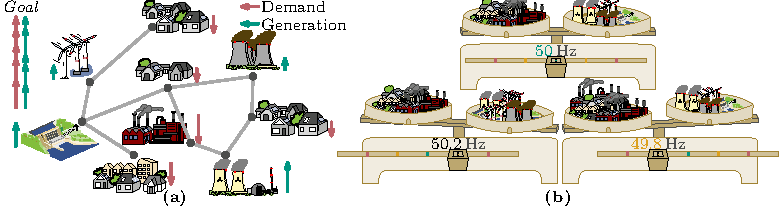
\includegraphics{foundations/figures/feasibility-problem.pdf}
    % 
    \caption[Simple description of the feasibility problem.]{The aim of the
    feasibility problem is to check whether the generation and demand are
    equivalent. This idea is shown by the two schematic sketches in (a) and (b).
    (a) gives a rough idea of the feasibility problem in terms of the power
    grid's generation and demand, (b) represents the same idea in the context of
    the (nominal) frequency of~\SI{50}{\glssymbol{hertz}} (top scale). The
    latter shows that any imbalance leads to a frequency that deviates from the
    nominal frequency in either way. If the generation is to high the frequency
    increases (bottom left scale). However, if the consumption is to high the
    frequency drops (bottom right scale).
    % 
    }%
    % 
    \label{ch:foundations:fig:feasibility-problem}
    % 
\end{figure}

Recall that the subproblem of any power grid analysis and thus, every placement
problem, is~\gls{feas}, \ie, whether there is a feasible power flow
for a given generation and demand. This problem is solved to check the
reliability of the power grid, to do short- and long-term planning (\ie,
placement problems; see~\cref{ch:switching,ch:facts}) and to solve other power
grid related problems. In this section, we will give an overview of the
different basic models, complexities, and relaxations.
% 
%%%%%%%%%%%%%%%%%%%%%%%%%%%%%%%%%%%%%%%%%%%%%%%%%%%%%%%%%%%%%%%%%%%%%%%%%%%%%%%%
\subsection{Alternating Current Power Flow Model}
\label{ch:foundations:sec:power-flow-analyses:subsec:AC-Model}
%%%%%%%%%%%%%%%%%%%%%%%%%%%%%%%%%%%%%%%%%%%%%%%%%%%%%%%%%%%%%%%%%%%%%%%%%%%%%%%%
% 
The~\acrlong{ac} (\gls{ac}) power flow models are the standard models for the
power flow analyses. Models are a description of the real-world that make
certain assumptions such that we have to explain why the models that we use are
reasonable for the problems that we tackle in this thesis. In this section, we
briefly introduce and describe~\gls{ac}~\gls{feas} that describes the power flow
in an~\gls{ac} power grid. We start with the dynamic~\gls{ac} model that is a
very precise model, but also a very complex model. Note that most placement
problems in power grids are long-term decisions. For long-term scenarios, it is
reasonable---since the power grid converges towards a stable state---to make an
assumption such that the~\gls{ac} model becomes time-independent
(see~\cref{ch:foundations:sec:power-flow-analyses:eq:complex-power-injection-resolution}).
The time-independent model is called~\emph{static}~\gls{ac} model. Using
different transformations, we derive different formulations
for~\gls{ac}~\gls{feas} shifting the non-convex and non-linear formulas in
different parts of the system of equations (see~\cref{tbl:ac-model-comparison}).
For problems that are long-term decisions these models are good approximations.
However, \gls{ac}~\gls{feas} is already~\NP-hard on star-shaped
networks~\parencite{Leh16}. In this work, we focus on high-voltage power grids
only, so we can make some assumption that lead to a linearization of~\gls{ac}
models. The linearization is called~\gls{dc}~\gls{feas}, which will be described
in the next section 
(\cref{ch:foundations:sec:power-flow-analyses:subsec:Lin-DC-Model}).

Typically, the theoretical structure of an~\gls{ac} model represents a
subproblem of different power grid problems that have to be solved within
different time ranges depending on the purpose. For instance, for power grid
planning (\ie, \acrlong{tnep}; in short~\gls{tnep}) the model has to be solved
every year~\parencite{Cai12}, whereas for day-ahead markets the particular model
has to be solved every day~\parencite{Cai12}. For the~\gls{ac} model there are
no known fast and robust solution techniques~\parencite{Cai12}, which is due to
the solver technologies not being able to guarantee global optimality since they
get stuck in local optima~\parencite[p.391;Chapter 18]{Fou96}.
% 
\begin{figure}[t!]
    % 
    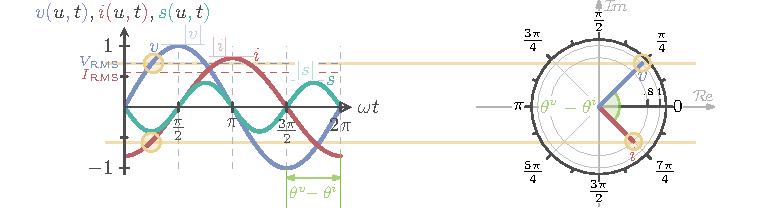
\includegraphics[page=1]{foundations/figures/ac-voltage-vs-current-angles.pdf}
    % 
    \caption[The relationship between voltage and current.]{
        The left side of the figure presents
        \textcolor{VOLTAGE}{voltage~$\textcolor{VOLTAGE}{\glssymbol{voltage}(
        \textcolor{TIMESTAMP}{\vertexa},\textcolor{TIMESTAMP}{\glssymbol{timestamp}})}$},
        \textcolor{CURRENT}
        {current~$\glssymbol{current}(\textcolor{TIMESTAMP}{\vertexa},
        \textcolor{TIMESTAMP}{\glssymbol{timestamp}})$},
        and~\textcolor{COMPLEXPOWER}{total instantaneous electric
        power}~$\textcolor{COMPLEXPOWER}{\glssymbol{complexpower}(\textcolor{TIMESTAMP}{\vertexa},\textcolor{TIMESTAMP}
        {\glssymbol{timestamp}})}$ in terms of trigonometric function for
        timestamp~$\textcolor{TIMESTAMP}{\glssymbol{timestamp}}\in\reals$ and
        vertex~$ \textcolor{TIMESTAMP} {\vertexa}\in\glssymbol{vertices}$. The
        Argand diagram is shown on the right side of the figure, where
        \textcolor{VOLTAGE}{voltage~$\glssymbol{voltage}(\textcolor{TIMESTAMP}{\vertexa},
        \textcolor{TIMESTAMP}{\glssymbol{timestamp}})$} and \textcolor{CURRENT}
        {current~$\glssymbol{current}(\textcolor{TIMESTAMP}{\vertexa},
        \textcolor{TIMESTAMP}{\glssymbol{timestamp}})$} are described by polar
        coordinates.
        % 
        The \textcolor{CURRENT}{current~$\glssymbol{current}(\textcolor{TIMESTAMP}{\vertexa},
        \textcolor{TIMESTAMP}{\glssymbol{timestamp}})$} is shifted
        by~\textcolor{POWERANGLE}{$\nicefrac{\gls{pi}}{2}$} to the right of
        \textcolor{VOLTAGE}{voltage~$\glssymbol{voltage}(\textcolor{TIMESTAMP}{\vertexa},
        \textcolor{TIMESTAMP}{\glssymbol{timestamp}})$} (\ie, voltage acts as
        reference point). The shift between voltage~$\glssymbol{voltage}(\textcolor{TIMESTAMP}{\vertexa},
        \textcolor{TIMESTAMP}{\glssymbol{timestamp}})$ and
        current~$\glssymbol{current}(\textcolor{TIMESTAMP}{\vertexa},
        \textcolor{TIMESTAMP}{\glssymbol{timestamp}})$ by~\textcolor{POWERANGLE}{$
        \glssymbol{voltageangle}-\glssymbol{currentangle}$}
        is also called~\textcolor{POWERANGLE}{power angle}. In the right diagram
        at timestamp~$\textcolor{TIMESTAMP}{\glssymbol{timestamp}} = 0$ the
        \textcolor{VOLTAGE}{voltage
        vector~$\glssymbol{voltage}(\textcolor{TIMESTAMP}{\vertexa},
        \textcolor{TIMESTAMP}{\glssymbol{timestamp}})$} completes a full cycle
        (\ie, a time period), whereas the \textcolor{CURRENT}{current
        vector~$\glssymbol{current}(\textcolor{TIMESTAMP}{\vertexa},
        \textcolor{TIMESTAMP}{\glssymbol{timestamp}})$} is on the negative
        imaginary axis and thus, lags behind the \textcolor{VOLTAGE}{voltage
        vector~$\glssymbol{voltage}(\textcolor{TIMESTAMP}{\vertexa},
        \textcolor{TIMESTAMP}{\glssymbol{timestamp}})$}
        by~\textcolor{POWERANGLE}{$\nicefrac{\gls{pi}}{2}$}. An inductive load
        could be a cause of that particular shift, since the
        \textcolor{VOLTAGE}{voltage~$\glssymbol{voltage}(\textcolor{TIMESTAMP}{\vertexa},
        \textcolor{TIMESTAMP}{\glssymbol{timestamp}})$} leads the
        \textcolor{CURRENT}{current~$\glssymbol{current}(\textcolor{TIMESTAMP}{\vertexa},
        \textcolor{TIMESTAMP}{\glssymbol{timestamp}})$}. The product of
        \textcolor{VOLTAGE}{voltage~$\glssymbol{voltage}(\textcolor{TIMESTAMP}{\vertexa},\textcolor{TIMESTAMP}{\glssymbol{timestamp}})$}
        and
        \textcolor{CURRENT}{current~$\glssymbol{current}(\textcolor{TIMESTAMP}{\vertexa},\textcolor{TIMESTAMP}{\glssymbol{timestamp}})$}
        is equivalent to the \textcolor{COMPLEXPOWER}{total instantaneous
        electric power}~$\textcolor{COMPLEXPOWER}{\glssymbol{complexpower}(
        \textcolor{TIMESTAMP}{\vertexa},\textcolor{TIMESTAMP}
        {\glssymbol{timestamp}})}$. Note that the magnitude of the
        total instantaneous
        electric power corresponds to the product of the~\acrlong{rms}
        (\gls{rms}) of the \textcolor{VOLTAGE}{voltage
        magnitude~$\fmagnitude{\glssymbol{voltage}(\textcolor{TIMESTAMP}{\vertexa})}$}
        denoted
        by~\textcolor{VOLTAGE}{\glssymbol{voltagerms}(\textcolor{TIMESTAMP}{\vertexa})}
        and the \textcolor{CURRENT}{current
        magnitude~$\fmagnitude{\glssymbol{current}(\textcolor{TIMESTAMP}{\vertexa})}$}
        denoted by~\textcolor{CURRENT}{
        \glssymbol{currentrms}(\textcolor{TIMESTAMP}{\vertexa})}. The derivation of this figure can be
        found
        in~\cref{ch:appendix:sec:fundamentals:sinusoid-plot-derivation}.
    %
    }%
    % 
    \label{ch:foundations:fig:AC-voltage-current-angle-difference}
    % 
\end{figure}
% 
\paragraph{Dynamic AC Model}
% 
The~\gls{ac} power flow in general consists of functions representing complex
current
injection~$\glssymbol{current}\colon\glssymbol{vertices}\times\reals\to\complexes$
and complex voltages injection~$\glssymbol{voltage}\colon
\glssymbol{vertices}\times\reals\to\complexes$ at a
vertex~$\vertexa\in\glssymbol{vertices}$ and timestamp~$\glssymbol{timestamp}\in\reals$ that are
sinusoid functions with amplitude~$\fmagnitude{\glssymbol{current}}$ and~$
\fmagnitude{\glssymbol{voltage}}$, respectively, angular
frequency~$\glssymbol{angularfrequency}\coloneqq\nicefrac{d\aangle}
{d\glssymbol{timestamp}}$ (\ie, \glssymbol{frequency} being the frequency; \eg,
\SI{50}{\glssymbol{hertz}} or~\SI{60}{\glssymbol{hertz}}), initial phases for
voltage and
current~$\glssymbol{voltageangle}\colon\glssymbol{vertices}\to\reals$
and~$\glssymbol{currentangle}\colon\glssymbol{vertices}\to\reals$, respectively,
and complex coefficients. 

The electrical power is defined by complex current~$\glssymbol{current}$ and
complex voltage~$\glssymbol{voltage}$ such that the complex
power~$\glssymbol{complexpower}(\vertexa,\glssymbol{timestamp})$ is defined
by~\cref{ch:foundations:sec:power-flow-analyses:eq:complex-power-vi}. 
% 
\begin{align}
    % 
    \glssymbol{complexpower}(\vertexa,\glssymbol{timestamp}) 
    % 
    &\coloneqq
    % 
    \glssymbol{voltage}(\vertexa,\glssymbol{timestamp})
    \cdot
    \conjugate{\glssymbol{current}(\vertexa,\glssymbol{timestamp})}
    &\qquad
    \forall
    \vertexa\in\glssymbol{vertices},
    \glssymbol{timestamp}\in\reals, 
    % 
    \label{ch:foundations:sec:power-flow-analyses:eq:complex-power-vi}
    % 
\end{align}
% 
where~$\conjugate{\glssymbol{current}(\vertexa,\glssymbol{timestamp})}$ is the complex
conjugate of the current. Since we use the complex conjugate of the current, we
get the relationship between voltage and current (see
also~\cref{ch:foundations:fig:AC-voltage-current-angle-difference}) that is the
difference between the voltage angle~\glssymbol{voltageangle} and the current
angle~\glssymbol{currentangle} meaning~$\glssymbol{voltageangle}-
\glssymbol{currentangle}$
(see~\cref{ch:foundations:sec:power-flow-analyses:eq:complex-power-injection-resolution}).
The latter difference is also called~\emph{power angle}. Thus, the function that
represents the complex power injection is defined
by~$\glssymbol{complexpower}\colon\glssymbol{vertices}\times\reals\to\complexes$.
% 
The real and imaginary part of a complex number~$z\in\complexes$ is denoted by~$
\real{z}$ and~$\imaginary{z}$, respectively. The voltage magnitude~$
\fmagnitude{\glssymbol{voltage}(\vertexa)}$
(\cref{ch:foundations:sec:power-flow-analyses:eq:voltage-magnitude}) represents
the wave crest (see left side
of~\cref{ch:foundations:fig:AC-voltage-current-angle-difference}) at
vertex~$\vertexa\in\glssymbol{vertices}$.
%
\begin{align}
    \fmagnitude{\glssymbol{voltage}(\vertexa)}
    &=
    \sqrt{\real{\glssymbol{voltage}(\vertexa,\glssymbol{timestamp})}^2 
    +
    \imaginary{\glssymbol{voltage}(\vertexa,\glssymbol{timestamp})}^2}.
    % 
    \label{ch:foundations:sec:power-flow-analyses:eq:voltage-magnitude}
\end{align}
% 
The current magnitude~$\fmagnitude{\glssymbol{current}(\vertexa)}$ is defined
accordingly
to~\cref{ch:foundations:sec:power-flow-analyses:eq:voltage-magnitude}. The
voltage and current magnitude are time independent,
since~\cref{ch:foundations:sec:power-flow-analyses:eq:voltage-magnitude} can be
written using trigonometric function~$\fmagnitude{\glssymbol{voltage}
(\vertexa)}\cdot$ $\sqrt{\cos^2
(\glssymbol{voltageangle}(\vertexa)+\glssymbol{angularfrequency}\glssymbol{timestamp})
+
\sin^2(\glssymbol{voltageangle}(\vertexa)+
\glssymbol{angularfrequency}\glssymbol{timestamp})}$, where the Pythagorean identity~$\sqrt{\cos^2
(\glssymbol{voltageangle}(\vertexa)+\glssymbol{angularfrequency}\glssymbol{timestamp}) +
\sin^2(\glssymbol{voltageangle}(\vertexa)+
\glssymbol{angularfrequency}\glssymbol{timestamp})} = 1$ follows from the complex plane
representation. 

% 
The idea behind this is that the assumption of time-invariance results in an
unchanging (\ie, constant) wave crest over time.
% 
If we assume that all functions are \emph{time-invariant}---having the same
behavior for the same input at any timestamp, \ie, the angular
frequency~$\nicefrac{d\aangle}{d\glssymbol{timestamp}} = \glssymbol{twopi}
\glssymbol{frequency}$ is constant---then we call them current and voltage
phasors. This allows us to use the phasor transform of Charles Proteus
Steinmetz~\parencite{Yan08,Rob12} such that we can use simple algebraic
equations on the phasors instead of differential equations of the sinusoid
signals. Note that the assumption of time-invariance might be acceptable for
some power flow analyses and planning problems. However, for smaller periods of
time such as the influence of switching processes on the grid stability this
assumption might not be suitable anymore. However, then we get into the range of
dynamic analyses~\parencite{Str18,Roh12,Tim14,Tim18}.

% 
We get the trigonometric relationship depicted
in~\cref{ch:foundations:sec:power-flow-analyses:eq:complex-power-injection-resolution}.
The derivation can be found
in~\cref{app:foundations:sec:power-flow-analyses:eq:complex-power-injection-resolution}.
%
\begin{subequations}
    \wormhole{bit:ch:foundations:sec:power-flow-analyses:eq:complex-power-injection-resolution} 
    \small
\begin{alignat}{2}
    \glssymbol{complexpower}(\vertexa,\timestamp) 
    &=
        \glssymbol{voltage}(\vertexa,\timestamp)
        \hspace{3.0cm}\cdot
        \conjugate{\glssymbol{current}(\vertexa,\timestamp)}
    \\
    &\begin{aligned}
        &=
        \hphantom{-\imgPart\cdot\big(}
        {\underbrace{
            \begin{aligned}
                \real{\glssymbol{voltage}(\vertexa,\timestamp)}
                \cdot
                \real{\glssymbol{current}(\vertexa,\timestamp)}
                +
                \imaginary{\glssymbol{voltage}(\vertexa,\timestamp)}
                \cdot
                \imaginary{\glssymbol{current}(\vertexa,\timestamp)}
            \end{aligned}
        }_{\eqqcolon\glssymbol{realpower}(\vertexa)}}%
        \\
        &\,\,\,\,-
        \imgPart\cdot
        {\underbrace{
            \begin{aligned}
                \big(
                    \real{\glssymbol{voltage}(\vertexa,\timestamp)}
                    \cdot
                    \imaginary{\glssymbol{current}(\vertexa,\timestamp)}
                    -
                    \imaginary{\glssymbol{voltage}(\vertexa,\timestamp)}
                    \cdot
                    \real{\glssymbol{current}(\vertexa,\timestamp)}
                \big)
            \end{aligned}
        }_{\eqqcolon\glssymbol{reactivepower}(\vertexa)}}%
    \end{aligned}%
    % 
    \label{ch:foundations:sec:power-flow-analyses:eq:complex-power:iv:rectangular}
    \\
    &=
        % \frac{1}{2}
        \fmagnitude{\glssymbol{voltage}(\vertexa)}
        \fmagnitude{\glssymbol{current}(\vertexa)} 
        \Big(
            \fcos{
                \glssymbol{voltageangle}(\vertexa) 
                + \angularfrequency\timestamp 
                - \glssymbol{currentangle}(\vertexa) 
                - \angularfrequency\timestamp
                } 
            +
            \imgPart\cdot
                \fsin{
                    \glssymbol{voltageangle}(\vertexa)  
                    + \angularfrequency\timestamp 
                    - \glssymbol{currentangle}(\vertexa)  
                    - \angularfrequency\timestamp
                    }
        \Big)
        \label{ch:foundations:sec:power-flow-analyses:eq:complex-power:iv:polar}
    \\
    &=
        \underbrace{
            % \frac{1}{2}
            \fmagnitude{\glssymbol{voltage}(\vertexa)}
            \fmagnitude{\glssymbol{current}(\vertexa)} 
            \fcos{\glssymbol{voltageangle}(\vertexa)
            - \glssymbol{currentangle}(\vertexa)} 
        }_{=\glssymbol{realpower}(\vertexa)}
        \hspace{16.7mm}+\hspace{0.5mm}
        \imgPart\cdot
        \underbrace{
            % \frac{1}{2}
            \fmagnitude{\glssymbol{voltage}(\vertexa)}
            \fmagnitude{\glssymbol{current}(\vertexa)}
            \fsin{\glssymbol{voltageangle}(\vertexa) - \glssymbol{currentangle}(\vertexa) } 
        }_{=\glssymbol{reactivepower}(\vertexa)}
        \label{ch:foundations:sec:power-flow-analyses:eq:complex-power:iv:polar:p:q}
    % 
\end{alignat}
    \label{ch:foundations:sec:power-flow-analyses:eq:complex-power-injection-resolution}
\end{subequations}
% 
Note that we have to use the~\acrlong{rms} (\gls{rms}) values
in~\cref{ch:foundations:sec:power-flow-analyses:eq:complex-power:iv:polar},
since $\fmagnitude{\glssymbol{voltage}(\vertexa)}\fmagnitude{\glssymbol{current}
(\vertexa)}$ would lead in a magnitude that is twice as high as of~$
\glssymbol{voltage}(\vertexa,\glssymbol{timestamp})\cdot\glssymbol{current}
(\vertexa,\glssymbol{timestamp})^\star$, which is graphically illustrated in~\cref{ch:foundations:fig:AC-voltage-current-angle-difference}. 
% 
To illustrate the time-varying power
in~\cref{ch:foundations:fig:AC-voltage-current-angle-difference}, we use the
concept of instantaneous electric power
(see~\cref{ch:appendix:sec:fundamentals:sinusoid-plot-derivation}), since the
complex power becomes time-independent
in~\cref{ch:foundations:sec:power-flow-analyses:eq:complex-power-injection-resolution}
and thus, constant. To illustrate the signals of the complex power a common way
is to use the real part of a signal (in our case the real part of the
current~\glssymbol{current} and voltage~\glssymbol{voltage},
see~\cref{ch:appendix:sec:fundamentals:sinusoid-plot-derivation} for more
details).

The penultimate step
in~\cref{ch:foundations:sec:power-flow-analyses:eq:complex-power-injection-resolution}
follows from the trigonometric addition and product formulas. In the last step,
the complex power equation becomes independent from time~\glssymbol{timestamp} and angle
frequency~\glssymbol{angularfrequency}. The intuition behind this is that in an
ideal~\gls{ac} network we start with the initial phase
angles~\glssymbol{voltageangle} and~\glssymbol{currentangle}, but the angular
frequency stays constant
meaning~$\glssymbol{angularfrequency}\coloneqq\nicefrac{d\aangle}{d\glssymbol{timestamp}} =
\glssymbol{twopi}\glssymbol{frequency}$. Thus, the rotation velocity is the same
for
both current and voltage. This simplifies the system such that it only depends
on the initial phases
(see~\cref{ch:foundations:fig:AC-voltage-current-angle-difference}) and leads
to a static analysis by using the resulting time-independent models that are
also called static models.
% 
\begin{figure}[t!]
    % 
    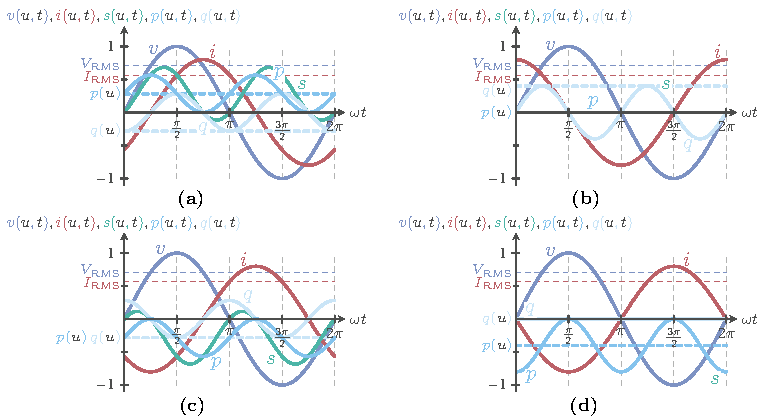
\includegraphics[page=1]{foundations/figures/ac-with-different-angles.pdf}
    % 
    \caption[Time varying~\gls{ac} sinusoid curves with different voltage angle
    differences.]{%
    % 
    The time varying sinusoid curves of
    \textcolor{VOLTAGE}{voltage~$\glssymbol{voltage}(\textcolor{TIMESTAMP}
    {\vertexa},\textcolor{TIMESTAMP}{\glssymbol{timestamp}})$}
    with
    magnitude~$\textcolor{VOLTAGE}{\fmagnitude{\glssymbol{voltage}(\textcolor{TIMESTAMP}
    {\vertexa}) }} = 1$ and effective
    value~$\textcolor{VOLTAGE}{\glssymbol{voltagerms}(\textcolor{TIMESTAMP}
    {\vertexa})} =
    \nicefrac{1}{\sqrt{2}}$, \textcolor{CURRENT}{current~$\glssymbol{current}(\textcolor{TIMESTAMP}
    {\vertexa},\textcolor{TIMESTAMP}{\glssymbol{timestamp}})$}
    with magnitude~$
    \textcolor{CURRENT}{\fmagnitude{\glssymbol{current}(\textcolor{TIMESTAMP}
    {\vertexa})}} = 0.8$ and effective
    value~$\textcolor{CURRENT}{\glssymbol{currentrms}(\textcolor{TIMESTAMP}
    {\vertexa})} =
    \nicefrac{0.8}{\sqrt{2}}$, \textcolor{COMPLEXPOWER}{total instantaneous
    electric
    power~$\glssymbol{complexpower}(\textcolor{TIMESTAMP}
    {\vertexa},\textcolor{TIMESTAMP}{\glssymbol{timestamp}})$}, its
    \textcolor{REALPOWER} {real
    part~$\glssymbol{realpower}(\textcolor{TIMESTAMP}{\vertexa},\textcolor{TIMESTAMP}{\glssymbol{timestamp}})$},
    and its \textcolor{REACTIVEPOWER}{imaginary part~$\glssymbol{reactivepower}(
    \textcolor{TIMESTAMP}{\vertexa},\textcolor{TIMESTAMP}{\glssymbol{timestamp}})$}
    are given for different voltage angle
    differences~\glssymbol{voltageangledifference}. The voltage angle
    differences are (a)~$\glssymbol{voltageangledifference} =
    \nicefrac{\gls{pi}}{4}$, (b)~$
    \glssymbol{voltageangledifference} = -\nicefrac{\gls{pi}}{2}$, (c)~$
    \glssymbol{voltageangledifference} = \nicefrac{3\gls{pi}}{4}$, and (d)~$
    \glssymbol{voltageangledifference} = \gls{pi}$. The 
    \textcolor{COMPLEXPOWER}{total instantaneous electric
    power~$\glssymbol{complexpower}(\textcolor{TIMESTAMP}
    {\vertexa},\textcolor{TIMESTAMP}{\glssymbol{timestamp}})$} is the sum of the
    \textcolor{REALPOWER}{real part~$\glssymbol{realpower}(\textcolor{TIMESTAMP}
    {\vertexa},\textcolor{TIMESTAMP}{\glssymbol{timestamp}})$} and the
    \textcolor{REACTIVEPOWER}{imaginary part~$\glssymbol{reactivepower}(
    \textcolor{TIMESTAMP} {\vertexa},\textcolor{TIMESTAMP}
    {\glssymbol{timestamp}})$} of the power. The same behavior is shown for
    the~\textcolor{COMPLEXPOWER}{complex
    power~$\glssymbol{complexpower}(\textcolor{TIMESTAMP}{\vertexa})$} and
    its~\textcolor{REALPOWER}{real power~$\glssymbol{realpower}(
    \textcolor{TIMESTAMP}{\vertexa})$} and~\textcolor{REACTIVEPOWER}{reactive
    power~$\glssymbol{reactivepower}(\textcolor{TIMESTAMP}{\vertexa})$}. (a)~A
    stable case is represented that is an operation of
    \textcolor{CURRENT}{current~\glssymbol{current}} and
    \textcolor{VOLTAGE}{voltage~\glssymbol{voltage}} within an angle shift
    of~$[-\nicefrac{\gls{pi}}{2};\nicefrac{\gls{pi}}{2}]$. (b)~One of the
    stability borders is~$-\nicefrac{\gls{pi}}{2}$, where the real part of the
    \textcolor{COMPLEXPOWER}{total instantaneous electric
    power~$\glssymbol{complexpower}(\textcolor{TIMESTAMP}
    {\vertexa},\textcolor{TIMESTAMP}{\glssymbol{timestamp}})$} is zero over
    \textcolor{TIMESTAMP}{time~$\glssymbol{timestamp}$}. (c)~With a voltage
    angle difference of~$\nicefrac{3\gls{pi}}{4}$ the power is within the
    instable section. All power curves are in the negative part. (d)~The
    \textcolor{CURRENT}{current~$\glssymbol{current}(\textcolor{TIMESTAMP}
    {\vertexa},\textcolor{TIMESTAMP}{\glssymbol{timestamp}})$} and
    \textcolor{VOLTAGE}{voltage~$\glssymbol{voltage}(\textcolor{TIMESTAMP}
    {\vertexa},\textcolor{TIMESTAMP}{\glssymbol{timestamp}})$} waves are in a
    state, where the waves cancel each other out. The reactive part of the total
    instantaneous electric power curve is zero and the real power part is
    negative. The derivation of this figure can be found
    in~\cref{ch:appendix:sec:fundamentals:sinusoid-plot-derivation}.
    % 
    }%
    % 
    \label{ch:foundations:fig:ac-with-different-angles}
    % 
\end{figure}
% Though the idealization of the angular frequency to a constant is for certain
% scenarios---as mentioned above---not suitable. 
\paragraph{Static AC Models}
% 
For general cases a common way to analyze power grids is to use a constant
angular frequency and analyze steady-state power grids that have one
fixed timestamp
per analysis. This will be our main focus in this work. However, the
idealization of the angular frequency to a constant is not suitable for certain
scenarios, as mentioned above. For this work it means that all previous
functions~$\mathbb{f}$ become time-independent~$\mathbb{f}\colon\mathbb{S}\to
\mathbb{F}$, where~$\mathbb{F}$ is a field and~$\mathbb{S}$ is the set we do the
mapping from such that for example the voltage function
becomes~$\glssymbol{voltage}\colon\glssymbol{vertices}\to\reals$.

\cref{ch:foundations:sec:power-flow-analyses:eq:complex-power:iv:polar} can be
rewritten to~$\glssymbol{complexpower}(\vertexa)\coloneqq\fmagnitude{\glssymbol{voltage}
(\vertexa)}\fmagnitude{\glssymbol{current}(\vertexa)}
e^{\imgPart\cdot(\glssymbol{voltageangle}(\vertexa) -
\glssymbol{currentangle}(\vertexa))}$ using Euler's formula. The
functions~$\glssymbol{realpower}\colon\glssymbol{vertices}\to\reals$
and~$\glssymbol{reactivepower}\colon\glssymbol{vertices}\to\reals$ represent the
\emph{real} and the \emph{reactive power}, respectively. This equation shows
very clearly the current angle~\glssymbol{currentangle} and voltage
angle~\glssymbol{voltageangle} that describe the real and reactive power on each
edge. \cref{ch:foundations:fig:AC-voltage-current-angle-difference} shows the
relationship of current~\glssymbol{current} and voltage~\glssymbol{voltage}. The
difference between voltage and current is the phase angle difference. The more
we increase the phase angle difference (\eg,
see~\cref{ch:foundations:fig:ac-with-different-angles} on
Page~\pageref{ch:foundations:fig:ac-with-different-angles}) between current and
voltage the smaller the real power gets until a certain point
(see~\cref{ch:foundations:fig:ac-with-different-angles}\screen{b}), where the
real power becomes zero. The case, where the wave crests of voltage and current
cancel each other out is shown
in~\cref{ch:foundations:fig:ac-with-different-angles}\screen{d}. Note that the
reactive power (also known as phantom power) increases while the real power
decreases, since current and voltage amplitudes do not decrease. The latter
basically describes the \emph{principle of conservation of energy}. The
described relationship between voltage, current, and power can be used to
maintain the voltage stability by changing real power demands. A decrease in
real power demand can be maintained by an increase in reactive power by changing
the phase angle difference between voltage and current. This mechanism helps to
maintain voltage on a certain level.

The complex power injection can be written in terms of real and reactive power
injection that represent decoupled parts
(see~\cref{ch:foundations:sec:power-flow-analyses:eq:complex-power-injection}
and its derivation
in~\cref{ch:foundations:sec:power-flow-analyses:eq:complex-power-injection-resolution}).
%   
\begin{align}
    \glssymbol{complexpower}(\vertexa) 
    % 
    = \real{\glssymbol{complexpower}(\vertexa)} 
    + \imgPart \cdot \imaginary{\glssymbol{complexpower}(\vertexa)} 
    % 
    = \glssymbol{realpower}(\vertexa) 
    + \imgPart \cdot \glssymbol{reactivepower}(\vertexa)
    % 
    \qquad
    \forall \vertexa\in\glssymbol{vertices}.
    % 
    \label{ch:foundations:sec:power-flow-analyses:eq:complex-power-injection}
\end{align}
% 
This relationship is shown
in~\cref{ch:foundations:fig:ac-with-different-angles}, where the total
instantaneous power~$\glssymbol{complexpower}(\vertexa,\glssymbol{timestamp})$
(respectively complex power~$\glssymbol{complexpower}(\vertexa)$) is the sum of
the real part~$\glssymbol{realpower} (\vertexa,\glssymbol{timestamp})$ and
imaginary part~$\glssymbol{reactivepower}(\vertexa,\glssymbol{timestamp})$ of
the power (respectively real power~$\glssymbol{realpower}(\vertexa)$ and
reactive power~$\glssymbol{reactivepower}(\vertexa)$). The total instantaneous
power curve~$\glssymbol{complexpower}(\vertexa,\glssymbol{timestamp})$
(respectively complex power~$\glssymbol{complexpower}(\vertexa)$) has the same
magnitude independent of the power angle. The latter emphasize the principle of
conservation of energy.

The real power~\glssymbol{realpower} is the power that is actually doing work
such as heating. However, reactive power is seldom consumed by consumers.
Exceptions are motors, generators and transformers that use a magnetic field
(inductive components) of industrial consumers that need reactive power. In
general reactive power is used to maintain the voltage stability. Increasing the
amount of reactive power increases the voltage that has to be kept in a certain
range. So reactive power is necessary for the power grid to have a more
efficient real power flow. The stability of the power grid is maintained by a
balance between real and reactive power and the latter depends highly on the
consumed real power.

We usually do a vertex-based analysis meaning that flows are usually modeled by
disturbance and injection at a vertex. We introduced for each vertex eight
variables denoted by~$\glssymbol{realpowergeneration}(\vertexa)$,
$\glssymbol{reactivepowergeneration}(\vertexa)$, $\glssymbol{realpowerdemand}
(\vertexa)$, $\glssymbol{reactivepowerdemand}(\vertexa)$,
$\glssymbol{voltage}(\vertexa)$, $\glssymbol{current}(\vertexa)$,
$\glssymbol{voltageangle}(\vertexa)$, and~$\glssymbol{currentangle}(\vertexa)$
for all~$\vertexa\in\glssymbol{vertices}$. However, we can always reformulate
current~$\glssymbol{current}$ and current angles~$\glssymbol{currentangle}$ in
terms of voltage~$\glssymbol{voltage}$ and voltage
angle~$\glssymbol{voltageangle}$ using Ohm's law and thus, we have just six
variables. We will see later that depending on the vertex type
(see~\cref{ch:foundations:tbl:load-flow-bus-specification}) or on the problem
some variables are given and thus, fixed to a certain value.

Up to now, we just looked at the power~\emph{injections} and not the
power~\emph{flows}. However, the complex, real, and reactive power flow, as well
as the complex current flow are defined by the
functions~$\glssymbol{complexpower}\colon\glssymbol{edges}\to\complexes$ (in
Volt Ampere; short~\SI{}{\gls{voltampere}}), $\glssymbol{realpower}\colon
\glssymbol{edges}\to\reals$ (in~\SI{}{\gls{watt}}),
$\glssymbol{reactivepower}\colon\glssymbol{edges}\to\reals$ (in Volt Ampere
Reactive; short~\SI{}{\gls{var}}), and~$\glssymbol{current}\colon
\glssymbol{edges}\to\complexes$ (in Ampere; short~\SI{}{\gls{ampere}}),
respectively. We distinguish between the injection at the source and sink vertex
of each edge, since there are power losses at each electrical element. 
% Depending
% on the problem statement, the above functions are usually unknown.
% 
\begin{figure}
    % 
    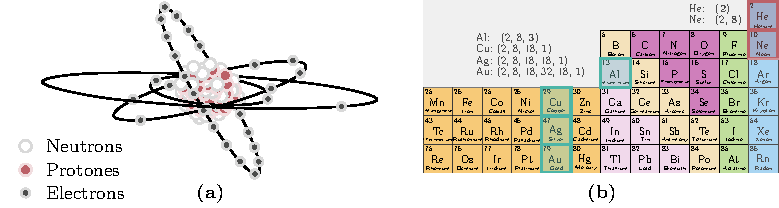
\includegraphics{foundations/figures/admittance.pdf}
    % 
    \caption[Relationship between conductivity and the material's atomic
    structure.]{Both (a) and (b) represent the atomic structure of one element
    and of multiple elements, respectively. The conductivity is dependent on the
    outermost shell denoted by valence shell. (a) The copper-$29$ isotope that
    has fully filled electron shells, but the valence shell (outermost shell).
    The valence shell has just one electron that is highly reactive. (b) Part of
    the description of the atomic structure of elements. The green marked
    elements represent common conductors and the red marked elements are strong
    insulators that are all in the last column.%
    }%
    % 
    \label{ch:foundations:sec:power-flow-analyses:fig:atomic-structure}
    % 
\end{figure}
% 
%%%%%%%%%%%%%%%%%%%%%%%%%%%%%%%%%%%%%%%%%%%%%%%%%%%%%%%%%%%%%%%%%%%%%%%%%%%%%%%%
\paragraph{Network Parameters}
\label{ch:foundations:network-parameters}
%%%%%%%%%%%%%%%%%%%%%%%%%%%%%%%%%%%%%%%%%%%%%%%%%%%%%%%%%%%%%%%%%%%%%%%%%%%%%%%%
% 
% 
The~\gls{ac}~network~\acnetworktuple is defined by the topological structure
that is given by the graph~$\glssymbol{graph} = (\glssymbol{vertices},
\glssymbol{edges})$,
the set~$\glssymbol{generators}\subseteq\glssymbol{vertices}$ of generators, the
set~$\glssymbol{consumers}\subseteq\glssymbol{vertices}$ of consumers,
% 
the resistance function~$\glssymbol{resistance}\colon
\glssymbol{undirectededges}\to\posreals\cup
\{\infty\}$,
% 
the reactance
function~$\glssymbol{reactance}\colon\glssymbol{undirectededges}\to\posreals\cup
\{\infty\}$,
% 
the susceptance
function~$\glssymbol{susceptance}\colon\glssymbol{undirectededges}\to\reals$~(\cref{ch:foundations:sec:power-flow-analyses:eq:susceptance}),
% 
the conductance function~$\glssymbol{conductance}\colon
\glssymbol{undirectededges}\to\reals$~(\cref{ch:foundations:sec:power-flow-analyses:eq:conductance}),
% 
the admittance
function~$\glssymbol{admittance}\colon\glssymbol{undirectededges}\to\complexes$~(\cref{ch:foundations:sec:power-flow-analyses:eq:admittance}),
% 
and the apparent power's thermal line limit
function~$\glssymbol{capacity}\colon\glssymbol{undirectededges}\to\reals$, which
can be either~$\glssymbol{currentmax}, \glssymbol{complexpowermax},
\glssymbol{realpowermax}$, or~$\glssymbol{reactivepowermax}$, and combinations
of them. The resistance~\glssymbol{resistance} and the
reactance~\glssymbol{reactance} are measured in Ohm~\gls{ohm}. The
admittance~$\glssymbol{admittance}(\vertexa,\vertexb)$~(\cref{ch:foundations:sec:power-flow-analyses:eq:admittance})
is defined by the
conductance~$\glssymbol{conductance}(\vertexa,\vertexb)$~(\cref{ch:foundations:sec:power-flow-analyses:eq:conductance})
and the
susceptance~$\glssymbol{susceptance}(\vertexa,\vertexb)$~(\cref{ch:foundations:sec:power-flow-analyses:eq:susceptance})
that defines how easy the current is able to flow through an element such as a
transmission line~$\{\vertexa,\vertexb\}\in\glssymbol{undirectededges}$. Note
that all three are measured in Siemens~\gls{siemens}. The conductivity of an
electrical element is mainly influenced by the conductance of the material,
length, and wire gauge. The conductance of the material is mainly influenced by
the atomic structure
(see~\cref{ch:foundations:sec:power-flow-analyses:fig:atomic-structure}).
Elements that have just one electron on the valence shell (\ie, outermost shell)
have a high conductivity such as copper, gold, and silver (Column 11 of the
periodic system;
see~\cref{ch:foundations:sec:power-flow-analyses:fig:atomic-structure}\screen{b}
green markers). However, elements that have a full valence shell are very good
insulators since the conductivity is very low, \eg, helium (last column of the
periodic system;
see~\cref{ch:foundations:sec:power-flow-analyses:fig:atomic-structure} red
markers). The admittance~\glssymbol{admittance},
impedance~\glssymbol{impedance}, conductance~\glssymbol{conductance}, and
susceptance~\glssymbol{susceptance} are defined
in~\crefrange{ch:foundations:sec:power-flow-analyses:eq:admittance}{ch:foundations:sec:power-flow-analyses:eq:susceptance}.
% 
\begin{align}
        \glssymbol{admittance}(\vertexa,\vertexc) 
&\coloneqq 
    \frac{1}{\glssymbol{impedance}(\vertexa,\vertexc)} =
    \glssymbol{conductance}(\vertexa,\vertexc) 
+ 
    \imgPart\cdot\glssymbol{susceptance}(\vertexa,\vertexc)
& \forall \{\vertexa,\vertexc\}\in\glssymbol{undirectededges},
% 
\label{ch:foundations:sec:power-flow-analyses:eq:admittance}
\\
    \glssymbol{impedance}(\vertexa,\vertexc) 
&\hphantom{:}=
    \frac{1}{\glssymbol{admittance}(\vertexa,\vertexc)} 
=
    \glssymbol{resistance}(\vertexa,\vertexc) 
+ 
    \imgPart\cdot\glssymbol{reactance}(\vertexa,\vertexc)
& \forall \{\vertexa,\vertexc\}\in\glssymbol{undirectededges},
% 
\label{ch:foundations:sec:power-flow-analyses:eq:impedance}
\\
    \glssymbol{conductance}(\vertexa,\vertexc) 
&\coloneqq
    \frac{\glssymbol{resistance}(\vertexa,\vertexc)}
    {\glssymbol{resistance}(\vertexa,\vertexc)^2 + \glssymbol{reactance}(\vertexa,\vertexc)^2}
& \forall \{\vertexa,\vertexc\}\in\glssymbol{undirectededges},
% 
\label{ch:foundations:sec:power-flow-analyses:eq:conductance}
\\
    \glssymbol{susceptance}(\vertexa,\vertexc) 
&\coloneqq 
    - \frac{\glssymbol{reactance}(\vertexa,\vertexc)}
    {\glssymbol{resistance}(\vertexa,\vertexc)^2 + \glssymbol{reactance}(\vertexa,\vertexc)^2}
& \forall \{\vertexa,\vertexc\}\in\glssymbol{undirectededges}.
% 
\label{ch:foundations:sec:power-flow-analyses:eq:susceptance}
\end{align}

Note that the admittance matrix~$\mathbf{\admittances}$ is defined by
the self-admittances representing the diagonal entries~$\glssymbol{admittance}
(\vertexa,\vertexa) = \glssymbol{admittance}(\vertexa,0) -
\sum_{\{\vertexa,\vertexc\}\in\glssymbol{undirectededges}}\glssymbol{admittance}
(\vertexa,\vertexc)$, where~$\glssymbol{admittance}(\vertexa,0)$ is the
admittance to ground, and the entries
of~\cref{ch:foundations:sec:power-flow-analyses:eq:admittance} that represent
the entries for the incident edge.
% 
%%%%%%%%%%%%%%%%%%%%%%%%%%%%%%%%%%%%%%%%%%%%%%%%%%%%%%%%%%%%%%%%%%%%%%%%%%%%%%%%
\paragraph{Power Grid Bounds}%
\label{ch:foundations:power-grid-bounds}
%%%%%%%%%%%%%%%%%%%%%%%%%%%%%%%%%%%%%%%%%%%%%%%%%%%%%%%%%%%%%%%%%%%%%%%%%%%%%%%%
% 
There are lower and upper bounds restricting the voltage angle
differences~$\glssymbol{voltageangledifferencemin}$
and~$\glssymbol{voltageangledifferencemax}$, the
voltages~\glssymbol{voltagemin}
and~\glssymbol{voltagemax}, the real power generation~
\glssymbol{realpowergenerationmin},
\glssymbol{realpowergenerationmax}, the reactive power
generation~\glssymbol{reactivepowergenerationmin},
\glssymbol{reactivepowergenerationmax},
the real power demand~\glssymbol{realpowerdemandmin},
\glssymbol{realpowerdemandmax}, and the reactive power
demand~\glssymbol{reactivepowerdemandmin},
\glssymbol{reactivepowerdemandmax}, respectively. The constraint of the voltage
angle difference (\cref{ch:foundations:eq-voltage-angle-difference-constraints})
restricts the power flow on each edge
(\cref{ch:foundations:sec:power-flow-analyses:eq:complex-power-injection-resolution}).
% 
\begin{subequations}
    \begin{alignat}{3}
        \glssymbol{voltageangledifferencemin}(\vertexa,\vertexc)
    &\leq
        \glssymbol{voltageangle}(\vertexa)
        &-&
        \glssymbol{voltageangle}(\vertexc)
    &\leq
        \glssymbol{voltageangledifferencemax}(\vertexa,\vertexc),
    % 
    \label{ch:foundations:sec:power-flow-analyses:eq:network:bounds:delta-voltageangle:polar}
    % 
    \\
    % 
        \glssymbol{voltageangledifferencemin}(\vertexa,\vertexc)
    &\leq
        \arctan
        \left(
            \frac{\imaginary{\glssymbol{voltage}(\vertexa)}}{\real{
            \glssymbol{voltage}(\vertexa)}}
        \right)
        &-&
        \arctan%
        \left(
            \frac{\imaginary{\glssymbol{voltage}(\vertexc)}}{\real{
            \glssymbol{voltage}(\vertexc)}}
        \right)
    &\leq
        \glssymbol{voltageangledifferencemax}(\vertexa,\vertexc),
    % 
    \label{ch:foundations:sec:power-flow-analyses:eq:network:bounds:delta-voltageangle:rectangular}
\end{alignat}
    \label{ch:foundations:eq-voltage-angle-difference-constraints}
\end{subequations}%
% 
for all~$\{\vertexa,\vertexc\}\in\glssymbol{undirectededges}$.
In~\cref{ch:foundations:sec:power-flow-analyses:eq:network:bounds:delta-voltageangle:rectangular},
we use the trigonometric relationship of the real part~$\real{
\glssymbol{voltage}(\vertexa)}$ and imaginary
part~$\imaginary{\glssymbol{voltage}(\vertexa)}$ that is defined by~$
\tan\big(\glssymbol{voltageangle}(\vertexa)\big) 
=
\nicefrac{
    \text{adjacent}
  }{
    \text{opposite}
  } 
= 
\nicefrac{
    \imaginary{\glssymbol{voltage}(\vertexa)}
  }{
    \real{\glssymbol{voltage}(\vertexa)}
  } 
= 
\nicefrac{
    \sin\big(\glssymbol{voltageangle}(\vertexa)\big)
  }{
    \cos\big(\glssymbol{voltageangle}(\vertexa)\big)
  }
$.
% 
The voltage angle difference is often restricted to the interval
of~$[-\nicefrac{\gls{pi}}{2};
\nicefrac{\gls{pi}}{2}]$ for stability reasons
(see~\cref{ch:foundations:fig:ac-with-different-angles} for different voltage
angle differences). If the balance between real power generation and demand
cannot be maintained (\ie, is not zero), then there is an issue in the angle
stability, \ie, the voltage angle difference cannot be maintained within the
stability interval. This in particular means the smaller the angle difference
the more balance between real power generation and demand exists. This is due to
the fact that the reactive power is used to compensate the lack of real power
generation and demand by shifting voltage and current using devices such as 
capacitor banks. \cref{ch:foundations:fig:ac-with-different-angles} explains why
exceeding the~$\nicefrac{\gls{pi}}{2}$ would lead to instabilities in the power
grid. Note that mainly generators are able to influence the voltage, power
curves, and the power angle
(see~\cref{ch:foundations:tbl:load-flow-bus-specification}). Thus, the network
stability is mainly driven by generators (including devices such as capacitor
banks). If the power angle exceeds the stability range the power curves shift
into the negative quadrant and the effective power values are negative, too
(see~\cref{ch:foundations:fig:ac-with-different-angles}\screen{b}--\screen{d}).
However, a power grid has a predefined flow direction and a negative real power
can be interpreted as a \textquote{backward power movement}
(see~\cref{ch:foundations:fig:ac-with-different-angles}\screen{a}).
% 
A rough idea of the latter is given by a simple~\gls{dc} circuit with a 
preinstalled diode. Note that a diode has a predefined direction making the
network nonreciprocal. The predefined direction defines the anode and cathode
for the battery connection. Connecting the battery in the wrong sense would lead
to a diode that does not flash.

In addition, the smaller the shift the less losses and the more stable the power
grid works.
In~\cref{ch:foundations:sec:power-flow-analyses:subsec:AC-vs-DC-Model}, we will
see that the differences are often smaller than~$\nicefrac{\gls{pi}}{6}$.
However, the voltage angle difference~$\glssymbol{voltageangledifference}$ also
correlates with the real power that flows from one vertex to another over the
power grid. The relationship becomes much clearer if we look at the
linearization of the~\gls{ac} model
in~\cref{ch:foundations:sec:power-flow-analyses:subsec:Lin-DC-Model}.

In some literature there is a constraint restricting the voltage
angles~$\glssymbol{voltageangle}(\vertexa)$ for
all~$\vertexa\in\glssymbol{vertices}$ themselves
(see~\cref{ch:foundations:sec:power-flow-analyses:eq:network:bounds:voltageangle}).
% 
\begin{equation}
    % \begin{align}
        \glssymbol{minvoltageangle}(\vertexa)
    \leq
        \glssymbol{voltageangle}(\vertexa)
    \leq
        \glssymbol{maxvoltageangle}(\vertexa)
    \qquad
    \forall
        \vertexa\in\glssymbol{vertices}.
    \label{ch:foundations:sec:power-flow-analyses:eq:network:bounds:voltageangle}
% \end{align}
\end{equation}
% 
The latter restricts the solution space and might exclude feasible solutions,
but does not represent a physical constraint. However, it improves the running
times to solve the feasibility problem and to fulfill assumptions such as the
stability range or later the
Assumption~\ref{ch:foundations:sec:power-flow-analyses:assumption:voltage-angle-difference}
in~\cref{ch:foundations:sec:power-flow-analyses:subsec:Lin-DC-Model}.

The voltage magnitude is bounded by
either~\cref{ch:foundations:sec:power-flow-analyses:eq:network:bounds:voltage-magnitude-min:polar},
or
by~\cref{ch:foundations:sec:power-flow-analyses:eq:network:bounds:voltage-magnitude-min:rectangular}
and~\cref{ch:foundations:sec:power-flow-analyses:eq:network:bounds:voltage-magnitude-max:rectangular}
depending on the formulation that is either polar or rectangular, respectively.
% 
\begin{subequations}
    \begin{alignat}{3}
        \fmagnitude{\glssymbol{voltagemin}(\vertexa)}\hphantom{)^2}
    &\leq
        &\fmagnitude{\glssymbol{voltage}(\vertexa)}
    &\leq&
        \fmagnitude{\glssymbol{voltagemax}(\vertexa)}\hphantom{)^2},
    % 
    \label{ch:foundations:sec:power-flow-analyses:eq:network:bounds:voltage-magnitude-min:polar}
    % 
    \\
        \glssymbol{voltagemin}(\vertexa)^2
    &\leq
        &\,\,\real{\glssymbol{voltage}(\vertexa)}^2
    +
        \imaginary{\glssymbol{voltage}(\vertexa)}^2,&&
    % 
    \label{ch:foundations:sec:power-flow-analyses:eq:network:bounds:voltage-magnitude-min:rectangular}
    % 
    \\
        &&\real{\glssymbol{voltage}(\vertexa)}^2 
    + 
        \imaginary{\glssymbol{voltage}(\vertexa)}^2\hphantom{,}
    &\leq&
        \glssymbol{voltagemax}(\vertexa)^2,
    % 
    \label{ch:foundations:sec:power-flow-analyses:eq:network:bounds:voltage-magnitude-max:rectangular}
\end{alignat}
\end{subequations}
% 
for all vertices~$\vertexa\in\glssymbol{vertices}$. This is mainly motivated by
the power grid elements that work within a certain voltage range. 
% 
% A usual range is~$\pm 5\%$ of the nominal voltage, where 
% 
Most elements perform poorly on the lower voltage end---\eg, inductive motors
over\-\mbox{heat---and} on the upper end the elements can get destroyed. The
thermal line limits can be represented in different ways that mainly depend on
the formulation. If the formulation uses current and
voltage, 
\cref{ch:foundations:sec:power-flow-analyses:eq:network:bounds:current-flow,ch:foundations:sec:power-flow-analyses:eq:network:bounds:current-flow:polar}
are used. Otherwise, if it uses real power, reactive power, and voltage
angles, 
\cref{ch:foundations:sec:power-flow-analyses:eq:network:bounds:complex-power-flow,ch:foundations:sec:power-flow-analyses:eq:network:bounds:complex-power:rectangular}
are used.
% 
\begin{subequations}
    \begin{alignat}{2}
    \{
        \glssymbol{current}(\vertexa,\vertexc)
        \in
        \complexes
    &\mid
        \real{\glssymbol{current}(\vertexa,\vertexc)}^2
    &+
        \imaginary{\glssymbol{current}(\vertexa,\vertexc)}^2
    &\leq
        \glssymbol{currentmax}(\vertexa,\vertexc)^2
    \},
    % 
    \label{ch:foundations:sec:power-flow-analyses:eq:network:bounds:current-flow}
    % 
    \\
    %
    &&
    \fmagnitude{\glssymbol{current}(\vertexa,\vertexc)} 
    &\leq 
    \glssymbol{currentmax}(\vertexa,\vertexc),
    %
    \label{ch:foundations:sec:power-flow-analyses:eq:network:bounds:current-flow:polar}
    % 
    \\
    % 
    \{ 
        \glssymbol{complexpower}(\vertexa,\vertexc)
        \in
        \complexes
    &\mid
        \real{\glssymbol{complexpower}(\vertexa,\vertexc)}^2 
    &+ 
        \imaginary{\glssymbol{complexpower}(\vertexa,\vertexc)}^2 
    % = 
    %     |\complexpower(\vertexa,\vertexc)|^2 
    &\leq
        \glssymbol{complexpowermax}(\vertexa,\vertexc)^2
    \},
    % 
    \label{ch:foundations:sec:power-flow-analyses:eq:network:bounds:complex-power-flow}
    \\
    %
    &&
    \fmagnitude{\glssymbol{complexpower}(\vertexa,\vertexc)} 
    &\leq 
    \glssymbol{complexpowermax}(\vertexa,\vertexc),
    %
    \label{ch:foundations:sec:power-flow-analyses:eq:network:bounds:complex-power:rectangular}
    %
\end{alignat}
\end{subequations}
% 
for all~$(\vertexa,\vertexc)\in\glssymbol{edges}$. Note that these
constraints are convex and quadratic as the geometric figure of its boundary is
a closed disk. In addition, the reactive power might increase the voltage
stability, but it also consumes bandwidth of the transmission line capacity.
Thus, to maximize the throughput of real power in the power grid the reactive
power has to be minimized such that the voltage stays in its range. Note that
increasing the real power decreases the losses.

The power injection constraints basically constrain the injection (\cref{ch:foundations:sec:power-flow-analyses:eq:network:bounds:real-power-injection,ch:foundations:sec:power-flow-analyses:eq:network:bounds:reactive-power-injection}) or
demand (\cref{ch:foundations:sec:power-flow-analyses:eq:network:bounds:real-power-disturbance,ch:foundations:sec:power-flow-analyses:eq:network:bounds:reactive-power-disturbance})
of a vertex depending on it being a generator or demand, respectively.
% 
\begin{subequations}
    \begin{align}
        \glssymbol{realpowergenerationmin}(\vertexa)
    &\leq
        \glssymbol{realpowergeneration}(\vertexa)
    \leq
        \glssymbol{realpowergenerationmax}(\vertexa) &
        \forall\vertexa\in\glssymbol{generators},
    % 
    \label{ch:foundations:sec:power-flow-analyses:eq:network:bounds:real-power-injection}
    \\
        \glssymbol{reactivepowergenerationmin}(\vertexa)
    &\leq
        \glssymbol{reactivepowergeneration}(\vertexa)
    \leq
        \glssymbol{reactivepowergenerationmax}(\vertexa) &
        \forall\vertexa\in\glssymbol{generators},
    % 
    \label{ch:foundations:sec:power-flow-analyses:eq:network:bounds:reactive-power-injection}
    \\
    % 
        \glssymbol{realpowerdemandmin}(\vertexa)
    &\leq
        \glssymbol{realpowerdemand}(\vertexa)
    \leq
        \glssymbol{realpowerdemandmax}(\vertexa)   & \forall\vertexa\in\glssymbol{consumers},
    % 
    \label{ch:foundations:sec:power-flow-analyses:eq:network:bounds:real-power-disturbance}
    \\
        \glssymbol{reactivepowerdemandmin}(\vertexa)
    &\leq
        \glssymbol{reactivepowerdemand}(\vertexa)
    \leq
        \glssymbol{reactivepowerdemandmax}(\vertexa)   &
        \forall\vertexa\in\glssymbol{consumers}.
    % 
    \label{ch:foundations:sec:power-flow-analyses:eq:network:bounds:reactive-power-disturbance}
\end{align}
    \label{ch:foundations:sec:power-flow-analyses:eq:injection-disturbance-bounds}
\end{subequations}
% 
The losses heavily depend on the voltage level
(\cref{ch:intro:fig:power-grid-structure}) and the amount of real power that
flow through an element.

Real power~\glssymbol{realpower} and voltage angles~\glssymbol{voltageangle}
strongly depend on each other, as well as reactive
power~\glssymbol{reactivepower} and voltage
magnitudes~$\fmagnitude{\glssymbol{voltage}}$
(see~\cref{ch:foundations:sec:power-flow-analyses:subsec:Lin-DC-Model}
Assumption~\ref{ch:foundations:sec:power-flow-analyses:assumption:voltage-magnitude}
with~\cref{ch:foundations:sec:power-flow-analyses:eq:assumption:vm}).
The~\realpowers-\glssymbol{voltageangle} and~\reactivepowers-\voltages problems
are weakly dependent on each other. Thus, the~\gls{ac} power flow is usually
solved in a decoupled way (see for example~\parencite{Gao18}). This is
reasonable if we follow the assumption that phase angle
differences~$\glssymbol{voltageangledifference}(\vertexa,\vertexb)$ are small
and high-voltage transmission lines are mainly reactive
meaning~$\glssymbol{resistance}
(\vertexa,\vertexb)\ll\glssymbol{reactance}(\vertexa,\vertexb)$ for all~$
\{\vertexa,\vertexb\}\in\glssymbol{undirectededges}$ (note that the latter
relationship is used in
Assumption~\ref{ch:foundations:sec:power-flow-analyses:assumption:negligible-resistance}
in~\cref{ch:foundations:sec:power-flow-analyses:subsec:Lin-DC-Model}). The
approach separates both subproblems and iterates between them. The decoupled
version decouples the~\gls{ac} power flow into two separate problems. However,
the full~\gls{ac} power flow includes both problems without these assumptions.
% 
\begin{table}[t!]
    \centering
    % latex table generated in R 3.2.2 by xtable 1.8-0 package
% Wed Jan 27 11:17:04 2016
{\setlength{\tabcolsep}{0.5em}}
{\renewcommand{\arraystretch}{1}}% for the vertical padding
\small
\begin{tabular}{
>{\centering\arraybackslash}m{1.6cm}
>{\centering\arraybackslash}m{0.2cm}
>{\centering\arraybackslash}m{2.25cm}
>{\centering\arraybackslash}m{2.25cm}
>{\centering\arraybackslash}m{0.5cm}
>{\centering\arraybackslash}m{2.85cm}
>{\centering\arraybackslash}m{0.6cm}
}
\toprule
%-------------------------------------------------------------------------------
  \multirow[c]{2}*{\textbf{Vertex Type}}     & 
  \multicolumn{4}{c}{\textbf{Variables}}  &
  \multirow[c]{2}*{\textbf{Comments}}     &
  \multirow[c]{2}*{\textbf{Code}}     \\
%-------------------------------------------------------------------------------
 \cmidrule(lr){2-5}
  & 
  \multicolumn{1}{c}{$\glssymbol{realpower}(\vertexa)$}     &
  \multicolumn{1}{c}{$\glssymbol{reactivepower}(\vertexa)$} & 
  \multicolumn{1}{c}{$\glssymbol{voltage}(\vertexa)$}   &
  \multicolumn{1}{c}{$\glssymbol{voltageangle}(\vertexa)$}       &
  \\
%-------------------------------------------------------------------------------
%-------------------------------------------------------------------------------
 \midrule  
%-------------------------------------------------------------------------------
   Load
   & \multicolumn{1}{c}{\textcolor{KITgreen}{\checkmark}}
   & \multicolumn{1}{c}{\textcolor{KITgreen}{\checkmark}}
   & \multicolumn{1}{c}{\textcolor{KITred}{\ding{55}}}
   & \multicolumn{1}{c}{\textcolor{KITred}{\ding{55}}}
   & \parbox{3cm}{Usual load representation}
   & \pqbus
  \\\addlinespace
%-------------------------------------------------------------------------------
  \rowcolor{Table-Line-Marker}
   Voltage Controlled 
   & \multicolumn{1}{c}{\textcolor{KITgreen}{\checkmark}} 
   & \multicolumn{1}{c}{\textcolor{KITred}{\ding{55}}} 
   & \multicolumn{1}{c}{\textcolor{KITgreen}{\checkmark}}
   & \multicolumn{1}{c}{\textcolor{KITred}{\ding{55}}} 
   & \parbox{3cm}{$\fmagnitude{\glssymbol{voltage}(\vertexa)}$ is held constant
   % no matter what~\reactances is
   }
   & \cvbus
  \\\addlinespace
%-------------------------------------------------------------------------------
   \vspace{1cm}\multirow{2}*{\shortstack[l]{Generator or\\ Synchronous\\
   Condenser}}
   & \multicolumn{1}{c}{\textcolor{KITgreen}{\checkmark}}
   & \multicolumn{1}{c}{\textcolor{KITred}{\ding{55}}}
   & \shortstack[l]{
      \multicolumn{1}{c}{\hspace*{-0.5cm}\textcolor{KITgreen}{\checkmark},}
      \\when \\$\glssymbol{reactivepowergenerationmin}(\vertexa)\! < \!
      \glssymbol{reactivepowergeneration}(\vertexa)\! < \!
      \glssymbol{reactivepowergenerationmax}(\vertexa)$
      }
   & \multicolumn{1}{c}{\textcolor{KITred}{\ding{55}}}
   &\vspace{-11mm}\multirow{2}*{\parbox{3cm}{\vspace{-4.5mm}
   Generator or synchronous 
   condenser ($\glssymbol{realpower}(\vertexa) = 0$) has~\si{\var} limits;
    % \hspace*{2.5mm}\reactivepowergenerationmin minimum~\si{\var} limit\\
    % \hspace*{2.5mm}\reactivepowergenerationmax maximum~\si{\var} limit\\
    $\fmagnitude{\glssymbol{voltage}(\vertexa)}$ is held as long
    as~\glssymbol{reactivepowergeneration}(\vertexa) and~\glssymbol{reactivepowerdemand}(\vertexa)
    are within limit}} &
    \vspace{1cm}\multirow{2}*{\pvbus}
  \\%
%-------------------------------------------------------------------------------
  \cmidrule(lr){2-5}
    & \textcolor{KITgreen}{\checkmark}
    & \shortstack[l]{
        \multicolumn{1}{c}{\hspace*{-0.9cm}\textcolor{KITgreen}{\checkmark},}\\
        when\\ 
        $-\glssymbol{reactivepowerdemandmax}(\vertexa)\! <\! 
        \glssymbol{reactivepowerdemand}(\vertexa) \!<\!
        -\glssymbol{reactivepowerdemandmin}(\vertexa)$
      }
    & \multicolumn{1}{c}{\textcolor{KITred}{\ding{55}}}
    & \multicolumn{1}{c}{\textcolor{KITred}{\ding{55}}}
    &% 
    &%bustype
   \\\addlinespace%
%-------------------------------------------------------------------------------
   \rowcolor{Table-Line-Marker}
   Fixed~\impedances to Ground
   & \multicolumn{1}{c}{\textcolor{KITred}{\ding{55}}}
   & \multicolumn{1}{c}{\textcolor{KITred}{\ding{55}}}
   & \multicolumn{1}{c}{\textcolor{KITred}{\ding{55}}}
   & \multicolumn{1}{c}{\textcolor{KITred}{\ding{55}}}
   & \parbox{3cm}{Only~\impedances is given}
   &%bustype
   \\\addlinespace%
%-------------------------------------------------------------------------------
   Reference, Slack & \multicolumn{1}{c}{\textcolor{KITred}{\ding{55}}} &
   \multicolumn{1}{c}{\textcolor{KITred}{\ding{55}}} &
   \multicolumn{1}{c}{\textcolor{KITgreen}{\checkmark}} &
   \multicolumn{1}{c}{\textcolor{KITgreen}{\checkmark}} &
   \parbox{3cm}{\emph{Swing bus} must adjust net power to hold voltage constant
   (essential for solution)} & 
   \vtbus
   \\%
%-------------------------------------------------------------------------------
    \rowcolor{Table-Line-Marker}
    Slack demand or tie
    & \multicolumn{1}{c}{\textcolor{KITred}{\ding{55}}}
    & \multicolumn{1}{c}{\textcolor{KITgreen}{\checkmark}}
    & \multicolumn{1}{c}{\textcolor{KITred}{\ding{55}}}
    & \multicolumn{1}{c}{\textcolor{KITgreen}{\checkmark}}
    & \parbox{3cm}{The \emph{tie} has no generation and demand attached}
    & \qtbus
    \\%
%-------------------------------------------------------------------------------
   \bottomrule
\end{tabular}

    % 
    \caption[Specification of the different power grid vertex types.]{This table
    is adopted from~\parencite[p.70; Figure~4.4]{wood1996power} and specifies
    the different vertex types in a power grid. The known variables at a
    vertex~$\vertexa\in\glssymbol{vertices}$ are marked by~\textcolor{KITgreen}
    {\checkmark} and the unknowns by~\textcolor{KITred}{\ding{55}}. Note that
    this table is for the~\pqv formulation of an~\gls{ac} model.    % The reference vertex is the vertex we
    % fix the voltage angle to a value.
    % 
    }
    % 
    \label{ch:foundations:tbl:load-flow-bus-specification}
\end{table}

Assuming that the demands are fixed, then out of the six variables~$
\glssymbol{voltageangledifference},\glssymbol{voltage}, 
\glssymbol{realpowergeneration}, \glssymbol{reactivepowergeneration},
\glssymbol{realpowerdemand}$, and~$\glssymbol{reactivepowerdemand}$ only four
remain. Each vertex specifies a certain type that is denoted by~\emph{vertex
type} that actually defines which variables are fixed. The common vertex types
are shown in~\cref{ch:foundations:tbl:load-flow-bus-specification}.
In~\cref{ch:network-analysis}, we describe the mathematical structure and
relationship of the linearized~\gls{ac} model. Within that structure it becomes
obvious why we chose exactly one vertex per connected component as slack vertex.
The basic idea is that a slack vertex represents a reference for the voltage
angles of the system and thus, choosing a voltage angle for that vertex defines
the voltage angles for all others.
In~\cref{ch:foundations:tbl:load-flow-bus-specification} there are exactly two
types that are able to work as slack vertex that are denoted by~\emph{slack}, or
\emph{slack demand}. The~\pqbus vertices are vertices without generation and
thus are, pure demand vertices. The~\pvbus is separated into two classes that
are both able to control voltage by adjusting the reactive power within certain
limits by either controlling the reactive power generation or demand. A source
of reactive power uses a capacitor such as a capacitor bank resulting in a
leading current flow by~$\nicefrac{\gls{pi}}{2}$ to voltage, whereas a sink of
reactive power uses an inductive device such as a coil resulting in a lacking
current flow by~$\nicefrac{\gls{pi}}{2}$. An example for the latter is given
in~\cref{ch:foundations:fig:AC-voltage-current-angle-difference}
and~\cref{ch:foundations:fig:ac-with-different-angles}. Note that reactive power
cannot be transmitted over long distances as the losses are too high. However,
the real and reactive power production is restricted by the generators operation
limits. If these limits are not sufficient to reach the voltage stability
additional equipment for reactive power is required. Another vertex that is able
to control voltage is the~\cvbus vertex that is either a special transformer
that is able to control its tap ratio or a~\gls{facts}.

The network parameters show the dependencies of the model and how complex it is
to maintain network stability in such networks. We already saw different
formulations of the complex~\gls{ac} model using either complex numbers or real
numbers with sinusoid functions. These non-linearities and the dependencies of
certain variables make the~\gls{ac} model hard to solve. In the following, we
describe the differences of these formulations.
% 
%%%%%%%%%%%%%%%%%%%%%%%%%%%%%%%%%%%%%%%%%%%%%%%%%%%%%%%%%%%%%%%%%%%%%%%%%%%%%%%%
\paragraph{Polar and Rectangular Formulations}
\label{ch:foundations:polar-rectangular-formulation}
%%%%%%%%%%%%%%%%%%%%%%%%%%%%%%%%%%%%%%%%%%%%%%%%%%%%%%%%%%%%%%%%%%%%%%%%%%%%%%%%
% 
In the previous part, we could see the different formulations of the voltage
angle differences and the power grid bounds. Depending on which formulation we
choose, we shift the complexity of the~\gls{ac} model to different parts as
shown in~\cref{tbl:ac-model-comparison}. We distinguish between
the~\emph{rectangular} and the~\emph{polar} formulation of the complex terms.

The polar formulation is given by the magnitude (\ie, length of the vector) and
the angle of its vector. We represented the complex power in its polar form
in~\cref{ch:foundations:sec:power-flow-analyses:eq:complex-power:iv:polar:p:q},
where~$\fmagnitude{\glssymbol{voltage}(\vertexa)}$ is the voltage magnitude
(also known as voltage amplitude) and~$\glssymbol{voltageangle}(\vertexa)$
represents the corresponding voltage angle.
% 
Contrary to that, the rectangular form of a complex number is given by the
real~$\real{\cdot}$ and imaginary part~$\imaginary{\cdot}$ of the complex number
representing the horizontal (x-axes) and vertical (y-axis) components in the
Argand diagram (\ie, geometric interpretation of a complex number;
see~\cref{ch:foundations:sec:power-flow-analyses:eq:complex-power:iv:rectangular}
and~\cref{ch:foundations:fig:AC-voltage-current-angle-difference} right side).
% 
In addition to that we are able to reformulate the power flow to calculate it in
terms of real power~\glssymbol{realpower}, reactive
power~\glssymbol{reactivepower}, and voltage~\glssymbol{voltage}. This
formulation is often denoted as~\pqv model
(see~\cref{app:foundations:sec:power-flow-analyses:eq:polar-pqv,app:foundations:sec:power-flow-analyses:eq:rectangular-pqv}).
Another alternative is the~\iv model that formulates the~\gls{ac} model in terms
of current~\glssymbol{current} and voltage~\glssymbol{voltage}
(see~\cref{app:foundations:sec:power-flow-analyses:eq:polar-iv,app:foundations:sec:power-flow-analyses:eq:rectangular-iv}).
We already saw parameter-dependent formulations in the power grid bounds part.

Note that the literature standard is the polar~\pqv
model~\parencite{wood1996power,Zimmerman2011} (see~\cref{app:foundations:sec:power-flow-analyses:eq:polar-pqv}).
% 
%%%%%%%%%%%%%%%%%%%%%%%%%%%%%%%%%%%%%%%%%%%%%%%%%%%%%%%%%%%%%%%%%%%%%%%%%%%%%%%%
\paragraph{PQV Formulations}
\label{ch:foundations:pqv-formulations}
%%%%%%%%%%%%%%%%%%%%%%%%%%%%%%%%%%%%%%%%%%%%%%%%%%%%%%%%%%%%%%%%%%%%%%%%%%%%%%%%
% 
The complex power injection at a vertex was introduced
in~\cref{ch:foundations:sec:power-flow-analyses:eq:complex-power:iv:polar:p:q}
using voltage and current as unknowns, which is denoted as~\iv formulation.
However, the formula can be restated to a complex power flow on an edge by
introducing the relationship that the current on an edge is defined
by~$
    % 
    \glssymbol{current}(\vertexa,\vertexc)
    \coloneqq
    \glssymbol{admittance}(\vertexa,\vertexc)
    \cdot
    \big(
        \glssymbol{voltage}(\vertexc) 
        - 
        \glssymbol{voltage}(\vertexa)
    \big)
    % 
$ for all~$(\vertexa,\vertexc)\in\glssymbol{edges}$. Using this relationship we
get~\cref{ch:foundations:sec:power-flow-analyses:eq:complex-power-flow:pqv} in
its rectangular formulation. The derivation can be found
in~\cref{app:foundations:sec:power-flow-analyses:eq:complex-power-flow-pqv-rectangular}.
% 
\begin{subequations}
    \small
\begin{alignat}{2}
    \glssymbol{complexpower}(\vertexa,\vertexc) 
    &=
    \glssymbol{voltage}(\vertexa)
    \cdot
    \glssymbol{current}(\vertexa,\vertexc)^\star 
    % 
    \label{ch:foundations:sec:power-flow-analyses:eq:complex-power-flow:pqv:rectangular:1}
    \\
    &= \glssymbol{voltage}(\vertexa)\cdot\glssymbol{admittance}
    (\vertexa,\vertexc)^\star\cdot
    \big(
        \glssymbol{voltage}(\vertexc)^\star
        - 
        \glssymbol{voltage}(\vertexa)^\star
    \big)
    % 
    \label{ch:foundations:sec:power-flow-analyses:eq:complex-power-flow:pqv:rectangular:2}
    \\
    &\begin{aligned}
        &\hphantom{=}
        \begin{rcases*}
            \!\!\!\!= \glssymbol{conductance}(\vertexa,\vertexc)
            \big(
                \real{\glssymbol{voltage}(\vertexa)}
                \real{\glssymbol{voltage}(\vertexc)}
                +
                \imaginary{\glssymbol{voltage}(\vertexa)}
                \imaginary{\glssymbol{voltage}(\vertexc)}
                -
                \real{\glssymbol{voltage}(\vertexa)}^2
                -
                \imaginary{\glssymbol{voltage}(\vertexa)}^2
            \big)
            \\
            +
            \glssymbol{susceptance}(\vertexa,\vertexc)
            \big(
                \real{\glssymbol{voltage}(\vertexc)}
                \imaginary{\glssymbol{voltage}(\vertexa)}
                -
                \real{\glssymbol{voltage}(\vertexa)}
                \imaginary{\glssymbol{voltage}(\vertexc)}
            \big)
        \end{rcases*} \eqqcolon \glssymbol{realpower}(\vertexa,\vertexc)
        \\
        &\,\,\,\,\hphantom{-}
        \begin{rcases*}
            \!\!\!\!+\imgPart
            \cdot
            \Big(
                \glssymbol{conductance}(\vertexa,\vertexc)
                \big(
                    \real{\glssymbol{voltage}(\vertexc)}
                    \imaginary{\glssymbol{voltage}(\vertexa)}
                    -
                    \real{\glssymbol{voltage}(\vertexa)}
                    \imaginary{\glssymbol{voltage}(\vertexc)}
                \big)
                \\
                % &\hspace{8mm}
                \!\!\!\!+
                \glssymbol{susceptance}(\vertexa,\vertexc)
                \big(
                    \real{\glssymbol{voltage}(\vertexa)}^2
                    +
                    \imaginary{\glssymbol{voltage}(\vertexa)}^2
                    -
                    \real{\glssymbol{voltage}(\vertexa)}
                    \real{\glssymbol{voltage}(\vertexc)}
                    -
                    \imaginary{\glssymbol{voltage}(\vertexa)}
                    \imaginary{\glssymbol{voltage}(\vertexc)}
                \big)
            \Big)
        \end{rcases*} \eqqcolon \glssymbol{reactivepower}(\vertexa,\vertexc)
        % 
        \label{ch:foundations:sec:power-flow-analyses:eq:complex-power-flow:pqv:rectangular}
        % 
    \end{aligned}
\end{alignat}
    \label{ch:foundations:sec:power-flow-analyses:eq:complex-power-flow:pqv}
\end{subequations}
% 
for all~$(\vertexa,\vertexc)\in\glssymbol{edges}$. The
rectangular~\cref{ch:foundations:sec:power-flow-analyses:eq:complex-power-flow:pqv:rectangular}
has only quadratic terms. It is possible to decompose the equation into the real
and reactive part of the complex power, which we already saw
in~\cref{ch:foundations:sec:power-flow-analyses:eq:complex-power:iv:polar:p:q,ch:foundations:sec:power-flow-analyses:eq:complex-power-injection}.
The real part can be transformed into the polar form
(see~\cref{ch:foundations:sec:power-flow-analyses:eq:real-power-flow:pqv:polar:full}).
% 
\begin{subequations}
    \begin{alignat}{2}
    \begin{split}
    \glssymbol{realpower}(\vertexa,\vertexc) 
    &= 
    \glssymbol{conductance}(\vertexa,\vertexc)
    \Big(
        \fmagnitude{\glssymbol{voltage}(\vertexa)}
        \fmagnitude{\glssymbol{voltage}(\vertexc)}
        \fcos{
            \glssymbol{voltageangle}(\vertexa) 
            - 
            \glssymbol{voltageangle}(\vertexc)
        }
        -
        \fmagnitude{\glssymbol{voltage}(\vertexa)}^2
    \Big)
    \\
    %%%%%%%%%%%%%%%%%%%%%%%%%%%%%%%%%%%%%%%%%%%%%%%%%%%%%%%%%%%%%%%%%%%%%%%%%%%
    &\,\,\,\,+ 
        \glssymbol{susceptance}(\vertexa,\vertexc)
        \fmagnitude{\glssymbol{voltage}(\vertexa)}
        \fmagnitude{\glssymbol{voltage}(\vertexc)}
        \fsin{
            \glssymbol{voltageangle}(\vertexa) 
            - 
            \glssymbol{voltageangle}(\vertexc) 
        }
    \end{split}
    %   
    \label{ch:foundations:sec:power-flow-analyses:eq:real-power-flow:pqv:polar}
    % 
\end{alignat}

    \label{ch:foundations:sec:power-flow-analyses:eq:real-power-flow:pqv:polar:full}
\end{subequations}
%
Similar, the reactive part can be transformed into the polar form (see~
\cref{ch:foundations:sec:power-flow-analyses:eq:reactive-power-flow:pqv:polar:full}).
% 
\begin{subequations}
    \begin{alignat}{2}
    \begin{split}
        \glssymbol{reactivepower}(\vertexa,\vertexc) 
        &= 
        \,\,\,\glssymbol{conductance}(\vertexa,\vertexc)
        \fmagnitude{\glssymbol{voltage}(\vertexa)}
        \fmagnitude{\glssymbol{voltage}(\vertexc)}
        \fsin{
            \glssymbol{voltageangle}(\vertexa) 
            - 
            \glssymbol{voltageangle}(\vertexc)
        }
    \\
        &\,\,\,\,-\glssymbol{susceptance}(\vertexa,\vertexc)
        \Big(
            \fmagnitude{\glssymbol{voltage}(\vertexa)}
            \fmagnitude{\glssymbol{voltage}(\vertexc)}
            \fcos{  
                \glssymbol{voltageangle}(\vertexa) 
                - 
                \glssymbol{voltageangle}(\vertexc) 
            }
            -
            \fmagnitude{\glssymbol{voltage}(\vertexa)}^2
        \Big)
    \end{split}
    % 
    \label{ch:foundations:sec:power-flow-analyses:eq:reactive-power-flow:pqv:polar}
    % 
\end{alignat}
    \label{ch:foundations:sec:power-flow-analyses:eq:reactive-power-flow:pqv:polar:full}
\end{subequations}
% 
The disadvantage of the polar formulations of the real and reactive power
in~\cref{ch:foundations:sec:power-flow-analyses:eq:real-power-flow:pqv:polar:full,ch:foundations:sec:power-flow-analyses:eq:reactive-power-flow:pqv:polar:full}
are the quadratic terms of the voltages and the trigonometric functions of the
voltage angle differences.
% 
%%%%%%%%%%%%%%%%%%%%%%%%%%%%%%%%%%%%%%%%%%%%%%%%%%%%%%%%%%%%%%%%%%%%%%%%%%%%%%%%
\paragraph{IV Formulation}
\label{ch:foundations:iv-formulations}
%%%%%%%%%%%%%%%%%%%%%%%%%%%%%%%%%%%%%%%%%%%%%%%%%%%%%%%%%%%%%%%%%%%%%%%%%%%%%%%%
% 
The~\gls{kcl} describes the flow of current at a vertex
(see~\cref{ch:foundations:sec:power-flow-analyses:eq:current-sum-at-vertex}). It
states that the net flow of current at each vertex is equal to zero that is
similar to the graph-theoretical conservation of flow shown
in~\cref{ch:foundations:sec:graph-theoretical-flows:eq:flow-conservation}.
% 
\begin{align}
    % 
    \glssymbol{current}(\vertexa) 
    \coloneqq
    \sum_{\vertexc\colon\{\vertexa,\vertexc\}\in\glssymbol{undirectededges}} 
    \glssymbol{current}(\vertexa,\vertexc)
    % 
    \qquad
    \forall\vertexa\in\glssymbol{vertices}.
    % 
    \label{ch:foundations:sec:power-flow-analyses:eq:current-sum-at-vertex}
    % 
\end{align}

The complex current can be restated in terms of voltages using Ohm's law. This
is shown
in~\cref{ch:foundations:sec:power-flow-analyses:eq:complex-current-ohm-voltage}
that is a linear function of complex voltages.
% 
\begin{align}
    \glssymbol{current}(\vertexa) 
    = 
    \glssymbol{admittance}(\vertexa,0)\cdot\glssymbol{voltage}(\vertexa)
    +
    \sum_{\{\vertexc\colon
    \{\vertexa,\vertexc\}\in\glssymbol{undirectededges}\mid\vertexa\not=\vertexc\}}
    \Big(
        \underbrace{
            \glssymbol{admittance}(\vertexa,\vertexc)
            (\glssymbol{voltage}(\vertexc) - \glssymbol{voltage}(\vertexa))
        }_{\eqqcolon\glssymbol{current}(\vertexa,\vertexc)}
    \Big)
    % 
    \qquad
    \forall\vertexa\in\glssymbol{vertices}
    % 
    \label{ch:foundations:sec:power-flow-analyses:eq:complex-current-ohm-voltage}
\end{align}
% 
The current injection~$\glssymbol{current}(\vertexa)$ at a
vertex~$\vertexa\in\glssymbol{vertices}$ is described by the voltage to
ground---using admittance to ground~$\glssymbol{admittance}(\vertexa,0)$---and
the current-based net flow. Note that the voltage to ground represents
disturbances at the vertex. The complex current flow can be rewritten into two
decoupled parts representing the real and imaginary part of the complex current
flow of an edge~$(\vertexa,\vertexc)\in\glssymbol{edges}$
(see~\cref{ch:foundations:sec:power-flow-analyses:eq:complex-current-flow-voltages}).
The derivation can be found
in~\cref{app:foundations:sec:power-flow-analyses:eq:complex-current-flow-rectangular}.
% 
\begin{align}
    \begin{array}{ll}  
    \glssymbol{current}(\vertexa,\vertexc) &= 
        \big(
            \glssymbol{conductance}(\vertexa,\vertexc) 
            + \imgPart\cdot\glssymbol{susceptance}(\vertexa,\vertexc)
        \big)
        \big(
            \glssymbol{voltage}(\vertexc) - \glssymbol{voltage}(\vertexa)
        \big)
    \\
    &=
        \Big(
            \glssymbol{conductance}(\vertexa,\vertexc) 
            + \imgPart\cdot\glssymbol{susceptance}(\vertexa,\vertexc)
        \Big)
        \Big(
            \real{\glssymbol{voltage}(\vertexc)} + \imgPart\cdot
            \imaginary{\glssymbol{voltage}
            (\vertexc)}
            - 
            \real{\glssymbol{voltage}(\vertexa)} - \imgPart\cdot
            \imaginary{\glssymbol{voltage}(\vertexa)}
        \Big)
    \\
    &
        \begin{aligned}
        =&
        &\underbrace{
            \glssymbol{conductance}(\vertexa,\vertexc)
            \big(
                \real{\glssymbol{voltage}(\vertexc)}-\real{\glssymbol{voltage}(\vertexa)}
            \big)
            -
            \glssymbol{susceptance}(\vertexa,\vertexc)
            \big(
                \imaginary{\glssymbol{voltage}(\vertexc)} - \imaginary{\glssymbol{voltage}(\vertexa)}
            \big)
        }_{\eqqcolon \realSmall{\glssymbol{current}(\vertexa,\vertexc)} }+
        \\
        &
        \imgPart\cdot
        \Big(
            &
            \underbrace{
                \glssymbol{conductance}(\vertexa,\vertexc)
                \big(
                    \imaginary{\glssymbol{voltage}(\vertexc)} - \imaginary{\glssymbol{voltage}(\vertexa)}
                \big)
                +
                \glssymbol{susceptance}(\vertexa,\vertexc)
                \big(
                    \real{\glssymbol{voltage}(\vertexc)} - \real{\glssymbol{voltage}(\vertexa)}
                \big)
            }_{\eqqcolon \imaginarySmall{\glssymbol{current}(\vertexa,\vertexc)} }
        \Big)
        \end{aligned}
\end{array}
    \label{ch:foundations:sec:power-flow-analyses:eq:complex-current-flow-voltages}
\end{align}
% 
More generally, we can write the problem of checking whether generation and
consumption agree as~\gls{ac}~\gls{feas}, which decision problem depends on the
formulation (see~\cref{tbl:ac-model-comparison}) and is defined in the following
problem box.
% 
\begingroup
    \begin{problem}[framed]{\acrlong{ac}~\acrlong{feas} $\acrshort{ac}~\gls{feas}
(\glssymbol{network})$}%
  Instance: & An \gls{ac} network~\acnetworktuple.\\
  % 
  Question: & Is there a feasible electrical flow complying with one of these
  model constraints in~\cref{tbl:ac-model-comparison}?
  % 
\end{problem}%
    \label{ch:fundamentals:problems:AC_FEAS-Decision_Problem}
\endgroup
% 
Summarizing the~\gls{ac}~\gls{feas} problem is a non-linear non-convex problem
that is under the assumption of time-invariance a model that is a good
approximation to a realistic power grid. Furthermore, it represents a subproblem
of all problems that have the power grid as an input.

\textcite{Leh16} discuss that the decoupled~\gls{ac} power flow model is weakly
\NP-hard on trees (stars). It represents a stronger result in terms of graph
classes, but includes real and reactive power as decoupled formulation. An
outline of the proof is given by~\textcite{Lav12}.
% 
%%%%%%%%%%%%%%%%%%%%%%%%%%%%%%%%%%%%%%%%%%%%%%%%%%%%%%%%%%%%%%%%%%%%%%%%%%%%%%%%
\paragraph{Normalization}%
\label{ch:foundations:sec:power-flow-analyses:normalization}
%%%%%%%%%%%%%%%%%%%%%%%%%%%%%%%%%%%%%%%%%%%%%%%%%%%%%%%%%%%%%%%%%%%%%%%%%%%%%%%%
% 
Note that for the power flow analysis it is common to normalize the system using
the~\glslongform{pu} (\glssymbol{pu}). The normalization is done for the complex power,
real power, reactive power, and voltage using the base units~\complexpowerbase,
\realpowerbase, \reactivepowerbase, and~\voltagebase, respectively. The other
units can be normalized by the bases derived from the previous power and voltage
base such that~$\currentbase = \nicefrac{\complexpowerbase}{\voltagebase}$,
$\impedancebase = \nicefrac{\voltagebase}{\currentbase}$, and~$\admittancebase =
\nicefrac{1}{\impedancebase}$.
% 
\begin{landscape}
\begin{table}[t!]
    \centering
    {\setlength{\tabcolsep}{0.3em}}
{\renewcommand{\arraystretch}{1}}% for the vertical padding
\small
% \begin{tabular}{p{2cm}p{3cm}p{3cm}p{3cm}p{3cm}p{3cm}}
\begin{tabular}{%
>{\centering\arraybackslash}m{2.4cm}%
>{\arraybackslash}m{1.9cm}%
>{\centering\arraybackslash}m{0.61cm}%
>{\arraybackslash}m{2cm}%
>{\centering\arraybackslash}m{0.61cm}%
>{\arraybackslash}m{2cm}%
>{\centering\arraybackslash}m{0.61cm}%
>{\arraybackslash}m{2cm}%
>{\centering\arraybackslash}m{0.61cm}%
>{\arraybackslash}m{1.5cm}%
>{\centering\arraybackslash}m{1.00cm}%
}%
% 
\toprule
  \multirow[c]{4}*{Constraints}   & 
  \multicolumn{4}{c}{Polar}       &
  \multicolumn{4}{c}{Rectangular} & 
  \multicolumn{1}{c}{DC}\\
%-------------------------------------------------------------------------------
%-------------------------------------------------------------------------------
 \cmidrule(lr){2-5}\cmidrule(lr){6-9}
  & 
  \multicolumn{2}{c}{PQV} &
  \multicolumn{2}{c}{IV}  &
  \multicolumn{2}{c}{PQV} & 
  \multicolumn{2}{c}{IV}  &
  \multicolumn{2}{c}{}
  \\
%-------------------------------------------------------------------------------
%-------------------------------------------------------------------------------
  \cmidrule(lr){2-3}\cmidrule(lr){4-5}\cmidrule(lr){6-7}\cmidrule(lr)
  {8-9}\cmidrule(lr){10-11}
   & 
   \multicolumn{1}{c}{Property}   &
   \multicolumn{1}{c}{Ref.}       &
   \multicolumn{1}{c}{Property}   & 
   \multicolumn{1}{c}{Ref.}       &
   \multicolumn{1}{c}{Property}   & 
   \multicolumn{1}{c}{Ref.}       &
   \multicolumn{1}{c}{Property}   & 
   \multicolumn{1}{c}{Ref.}       &
   \multicolumn{1}{c}{Property}   & 
   \multicolumn{1}{c}{Ref.}
   \\
%-------------------------------------------------------------------------------
%-------------------------------------------------------------------------------
 \midrule  
%-------------------------------------------------------------------------------
%-------------------------------------------------------------------------------
  \rowcolor{Table-Line-Marker}%
  \textbf{Network Flow}%
    & Quadratic equation and trigonometric functions%
    & 
    % \ref{ch:foundations:sec:power-flow-analyses:eq:complex-power-flow:pqv},
    \ref{ch:foundations:sec:power-flow-analyses:eq:real-power-flow:pqv:polar:full},
    \ref{ch:foundations:sec:power-flow-analyses:eq:reactive-power-flow:pqv:polar:full}.
    & Quadratic equation and trigonometric functions%
    & 
    based on
    \ref{ch:foundations:sec:power-flow-analyses:eq:complex-current-ohm-voltage},
    \ref{ch:foundations:sec:power-flow-analyses:eq:complex-current-flow-voltages}.
    & Quadratic equations%
    & 
    \ref{ch:foundations:sec:power-flow-analyses:eq:complex-power-flow:pqv:rectangular}.
    & Linear \mbox{constraints}%
    & 
    \ref{ch:foundations:sec:power-flow-analyses:eq:current-sum-at-vertex},
    \ref{ch:foundations:sec:power-flow-analyses:eq:complex-current-ohm-voltage},
    \ref{ch:foundations:sec:power-flow-analyses:eq:complex-current-flow-voltages}.
    & Linear equations
    & 
    \ref{ch:foundations:sec:power-flow-analyses:dc:eq:kvl}
    \\
  \textbf{Voltage Angle Difference}~$\deltaangle$  %line         
    & Linear \mbox{constraints}
    & 
    
    \ref{ch:foundations:sec:power-flow-analyses:eq:network:bounds:delta-voltageangle:polar}.
    & Linear \mbox{constraints}
    & 
    \ref{ch:foundations:sec:power-flow-analyses:eq:network:bounds:delta-voltageangle:polar}.
    & Non-convex \mbox{constraints} with trigonometric functions
    & 
    \ref{ch:foundations:sec:power-flow-analyses:eq:network:bounds:delta-voltageangle:rectangular}.
    & Non-convex \mbox{constraints} with trigonometric functions
    & 
    \ref{ch:foundations:sec:power-flow-analyses:eq:network:bounds:delta-voltageangle:rectangular}.
    & Linear \mbox{constraints}
    & 
    \ref{ch:foundations:sec:power-flow-analyses:dc:eq:angle-difference}.
    \\
  \rowcolor{Table-Line-Marker}
  \textbf{Vertices \& Edges}
    & Linear \mbox{constraints}
    & 
    \ref{ch:foundations:sec:power-flow-analyses:eq:network:bounds:voltage-magnitude-min:polar},
    \ref{ch:foundations:sec:power-flow-analyses:eq:injection-disturbance-bounds}.
    & Linear \mbox{constraints}
    & 
    \ref{ch:foundations:sec:power-flow-analyses:eq:network:bounds:voltage-magnitude-min:polar},
    \ref{ch:foundations:sec:power-flow-analyses:eq:network:bounds:current-flow},
    
    \ref{ch:foundations:sec:power-flow-analyses:eq:network:bounds:current-flow:polar},
    \ref{ch:foundations:sec:power-flow-analyses:eq:complex-power:iv:polar:p:q}
    ineq.
    & Quadratic inequalities (some non-convex)
    & 
    \ref{ch:foundations:sec:power-flow-analyses:eq:network:bounds:voltage-magnitude-min:rectangular},
    \ref{ch:foundations:sec:power-flow-analyses:eq:network:bounds:voltage-magnitude-max:rectangular},
    \ref{ch:foundations:sec:power-flow-analyses:eq:complex-power:iv:rectangular} %
    with %
    \ref{ch:foundations:sec:power-flow-analyses:eq:network:bounds:current-flow}.%
    & Quadratic inequalities (some non-convex)
    & 
    \ref{ch:foundations:sec:power-flow-analyses:eq:network:bounds:voltage-magnitude-min:rectangular},
    \ref{ch:foundations:sec:power-flow-analyses:eq:network:bounds:voltage-magnitude-max:rectangular},
    \ref{ch:foundations:sec:power-flow-analyses:eq:network:bounds:current-flow:polar}.%
    & Linear \mbox{constraints}
    & 
    \ref{ch:foundations:sec:power-flow-analyses:dc:eq:kcl}--\ref{ch:foundations:sec:power-flow-analyses:dc:eq:capacity}
    \\ 
  \textbf{Models}
    & \multicolumn{2}{c}{\cref{app:foundations:sec:power-flow-analyses:eq:polar-pqv} }
    & \multicolumn{2}{c}{\cref{app:foundations:sec:power-flow-analyses:eq:polar-iv} }
    & \multicolumn{2}{c}{\cref{app:foundations:sec:power-flow-analyses:eq:rectangular-pqv} }
    & \multicolumn{2}{c}{\cref{app:foundations:sec:power-flow-analyses:eq:rectangular-iv} }
    & \multicolumn{2}{c}{\crefrange{ch:foundations:sec:power-flow-analyses:dc:eq:kcl}{ch:foundations:sec:power-flow-analyses:dc:eq:angle-difference} }
    \\
%-------------------------------------------------------------------------------
%-------------------------------------------------------------------------------
%-------------------------------------------------------------------------------
   \bottomrule
\end{tabular}

    % 
    \caption[Comparison of the different~\acrshort{ac} models.]{This table is
    inspired by~\textcite{Cai12} from~\gls{ferc} that analyzed~\gls{acopf} and
    compares the different~\gls{ac} models. The columns represent different
    constraint types that are related with the network flow, voltage angle
    differences, and vertices. For each formulation, the property describes the
    complexity of the constraint and the Ref. represents the equation's
    reference number either in this chapter or for some of the complete models
    in the appendix. }
    % 
    \label{tbl:ac-model-comparison}
\end{table}
\end{landscape}
% 
%%%%%%%%%%%%%%%%%%%%%%%%%%%%%%%%%%%%%%%%%%%%%%%%%%%%%%%%%%%%%%%%%%%%%%%%%%%%%%%%
\paragraph{Transmission Line Representation}
\label{ch:foundations:sec:power-flow-analyses:transmission-line-representation}
%%%%%%%%%%%%%%%%%%%%%%%%%%%%%%%%%%%%%%%%%%%%%%%%%%%%%%%%%%%%%%%%%%%%%%%%%%%%%%%%
% 
We use transmission line representations (also known as branch or transmission
line models) to simplify the power flow analysis to a purely vertex-based
analysis using the admittances between adjacent vertices
(see~\cref{ch:foundations:sec:power-flow-analyses:eq:complex-power-flow:pqv:rectangular:2,ch:foundations:sec:power-flow-analyses:eq:complex-current-ohm-voltage}).%
\begin{figure}
    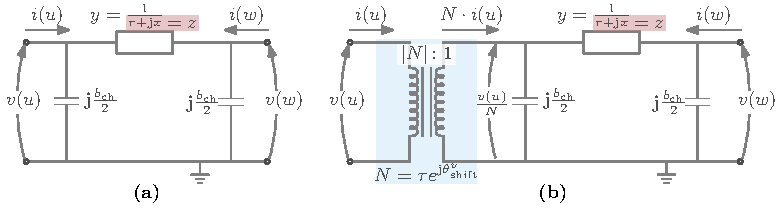
\includegraphics{foundations/figures/pi-equivalent-circuit.pdf}
    % 
    \caption[The Pi-equivalent circuit model for a transmission line]{The
    Pi-equivalent circuit represents a model of a transmission line with medium
    length. Note that this figure is partly adopted from~\textcite[p.17; Figure
    3-1]{Zimmerman2011}. (a)\&(b) The two capacitors model the transmission
    line charging~$\glssymbol{linechargingsusceptance}$, the
    impedance~\glssymbol{impedance} models the resistive behavior of a
    transmission line (red). (b) If the line represents a phase shift
    transformer then the transformer is modeled on one of the two end vertices
    (blue). The transformer (blue) is usually modeled at the vertex with the
    primary coil with a fix tap ratio~\glssymbol{tapratio} and in that
    particular case with a fix phase shift angle~\glssymbol{voltageangleshift}.
    The voltage~\glssymbol{voltage} and current~\glssymbol{current} change with
    respect to the number of windings~$\fmagnitude{N}$ on the side of the
    secondary coil. }
    % 
    \label{ch:foundations:sec:power-flow-analyses:fig:pi-equivalent-circuit}
    % 
\end{figure}
% 

For the model formulation of the previous part of this section, we used a single
line model and considered a transmission line model that is denoted
by~\emph{short transmission line representation} that neglects shunt elements
such as the shunt capacitance~\glssymbol{linechargingsusceptance} representing
the charging of a line
(see~\cref{ch:foundations:sec:power-flow-analyses:fig:pi-equivalent-circuit}).
The short transmission line representation approximates lines that are up to
80~\si{km} long by using a similar model as the RLC circuit, meaning resistance,
impedance, and capacitance are in series (see also Kirchhoff's~\nth{3}
postulate~\parencite[p.127]{Ses61}). Note that the assumption for the short
transmission line representation is reasonable, since the line charging is
negligible. Within the~\gls{ac} model terminology, we often model
the~\emph{shunt conductance} and~\emph{shunt susceptance} as elements connected
to the vertices. These elements are purely model-based theoretical elements used
to model elements such as transmission lines or synchronous condensers.
Depending on which transmission line representation is used, the shunt elements
are included or not.

For high voltage power grids it is more common to model the transmission lines
using the~\emph{medium line approximation} that includes a lumped shunt
admittance. There are two different models denoted by~\emph{pi representation}
% 
(see~\cref{ch:foundations:sec:power-flow-analyses:fig:pi-equivalent-circuit}\screen{(a)}) 
% 
and~\emph{T representation}. \textcite[p.75]{wood1996power} and applications
such as Matpower~\parencite[pp.16ff.]{Zimmerman2011} and
Pypower~\parencite{online:pypower} use the pi representation. However, there is
much more investigation in this topic as can be seen by~\textcite{CANO201771},
who introduce different transmission line representations. Note that the
standard pi representation does not include transformers (see the next
paragraph on transmission line elements).
% 
In~\cref{ch:foundations:sec:power-flow-analyses:fig:pi-equivalent-circuit}\screen{(b)},
% 
we can see the pi representation with a tap transformer. Note that there are
also~\emph{long line approximations} that are not considered in this work.
However, the pi representation is the standard model for medium length
transmission lines that are up to~$250$~\si{\km} long, which is a realistic
assumption for~\gls{ac} models. Note that most of the transmission lines are up
to 100~\si{\km} long~\parencite[p.112]{Nov12}.

The line charging
susceptance~$\glssymbol{linechargingsusceptance}(\vertexa,\vertexc)$ is a parameter of a
transmission line~$\{\vertexa,\vertexc\}\in\glssymbol{undirectededges}$ as
medium to long transmission lines tend to have an inherent capacitance. The pi
model provides us with the ability to introduce the
impedance~$\glssymbol{impedance}(\vertexa,\vertexc)$ and line charging
susceptance~$\glssymbol{linechargingsusceptance}(\vertexa,\vertexc)$ to the
admittances~$\glssymbol{admittance}(\vertexa,\vertexc)$ for all~$
\{\vertexa,\vertexc\}\in\glssymbol{undirectededges}$ and use the standard power
flow analysis as shown in the previous part of this section. The only difference
are the charge elements in the complex power equations
(see~\cref{ch:foundations:sec:power-flow-analyses:eq:complex-power-flow:pi-model}).
%
\begin{subequations}
    % \small
\begin{align}
    &\realpower(\vertexa,\vertexc) + \imgPart\cdot\reactivepower(\vertexa,\vertexc)
\\ 
% 
&=  \glssymbol{voltage}(\vertexa)
    \Big( 
        \big(
            \glssymbol{voltage}(\vertexa) - \glssymbol{voltage}(\vertexc)
        \big)
        \admittance(\vertexa,\vertexc)
    \Big)^\star 
    +
    \glssymbol{voltage}(\vertexa)
    \big(
        \glssymbol{voltage}(\vertexa)\linechargingadmittance(\vertexa, \vertexc)
    \big)^\star
\\%
%
&\begin{aligned}
&=  \fmagnitude{\glssymbol{voltage}(\vertexa)}e^{\imgPart\cdot\glssymbol{voltageangle}(\vertexa)} 
    \left( 
        \left(
            \fmagnitude{\glssymbol{voltage}(\vertexa)}e^{\imgPart\cdot\glssymbol{voltageangle}(\vertexa)} 
            - 
            \fmagnitude{\glssymbol{voltage}(\vertexc)}e^{\imgPart\cdot\glssymbol{voltageangle}(\vertexc)} 
        \right) 
        \left( 
            \conductance(\vertexa,\vertexc) 
            + 
            \imgPart\cdot\glssymbol{susceptance}(\vertexa,\vertexc) 
        \right) 
    \right)^\star 
    \\
    &\,\,\,\,- 
    \imgPart\cdot|\glssymbol{voltage}(\vertexa)|^2 \linechargingsusceptance(\vertexa,\vertexc)
\end{aligned}
\\%
% 
&\begin{aligned}
&=  \left( 
        \fmagnitude{\glssymbol{voltage}(\vertexa)}^2 
        - 
        \fmagnitude{\glssymbol{voltage}(\vertexa)}\cdot\fmagnitude{\glssymbol{voltage}(\vertexc)} 
        \cos 
        \left(
            \glssymbol{voltageangle}(\vertexa) - \glssymbol{voltageangle}(\vertexc)
        \right) 
        - 
        \imgPart\cdot\fmagnitude{\glssymbol{voltage}(\vertexa)}\fmagnitude{\glssymbol{voltage}(\vertexc)}
        \sin
        \left( 
            \glssymbol{voltageangle}(\vertexa) - \glssymbol{voltageangle}(\vertexc) 
        \right)
    \right) 
    \\
    &\times 
    \left(
            \conductance(\vertexa,\vertexc) 
            + 
            \imgPart\cdot\glssymbol{susceptance}(\vertexa,\vertexc) 
    \right)^\star 
    - \imgPart\cdot\fmagnitude{\glssymbol{voltage}(\vertexa)}^2 \linechargingsusceptance(\vertexa,\vertexc)
\end{aligned}
\end{align}
    \small
\begin{alignat}{2}
    &\glssymbol{realpower}(\vertexa,\vertexc) + \imgPart\cdot\glssymbol{reactivepower}(\vertexa,\vertexc)
\\ 
% 
&=  \glssymbol{voltage}(\vertexa)
    \Big( 
        \big(
            \glssymbol{voltage}(\vertexa) - \glssymbol{voltage}(\vertexc)
        \big)
        \glssymbol{admittance}(\vertexa,\vertexc)
    \Big)^\star 
    +
    \glssymbol{voltage}(\vertexa)
    \big(
        \glssymbol{voltage}(\vertexa)\glssymbol{linechargingadmittance}(\vertexa, \vertexc)
    \big)^\star
% \\%
% %
% &\begin{aligned}
% &=  \fmagnitude{\glssymbol{voltage}(\vertexa)}e^{\imgPart\cdot\glssymbol{voltageangle}(\vertexa)} 
%     \left( 
%         \left(
%             % \frac{1}{\imgPart\reactance\tapratio^2}
%             \fmagnitude{\glssymbol{voltage}(\vertexa)}
%             e^{\imgPart\cdot\glssymbol{voltageangle}(\vertexa)} 
%             - 
%             % \frac{1}{\tapratio\reactance e^{-\imgPart\cdot\glssymbol{voltageangle}shift} }
%             \fmagnitude{\glssymbol{voltage}(\vertexc)}
%             e^{\imgPart\cdot\glssymbol{voltageangle}(\vertexc)} 
%         \right) 
%         % \left( 
%         %     \conductance(\vertexa,\vertexc) 
%         %     + 
%         %     \imgPart\cdot\glssymbol{susceptance}(\vertexa,\vertexc) 
%         % \right) 
%         \glssymbol{linechargingadmittance}(\vertexa,\vertexc)
%     \right)^\star 
%     % \\
%     % &\,\,\,\,
%     - 
%     \imgPart\cdot\fmagnitude{\glssymbol{voltage}(\vertexa)}^2
%     \glssymbol{linechargingsusceptance}(\vertexa,\vertexc)
% \end{aligned}
\\%
% 
&\begin{aligned}
&=  \Big( 
        \fmagnitude{\glssymbol{voltage}(\vertexa)}^2 
        - 
        \fmagnitude{\glssymbol{voltage}(\vertexa)}\cdot\fmagnitude{\glssymbol{voltage}(\vertexc)} 
        \cos 
        \left(
            \glssymbol{voltageangle}(\vertexa) - \glssymbol{voltageangle}(\vertexc)
        \right) 
        - 
        \imgPart\cdot\fmagnitude{\glssymbol{voltage}(\vertexa)}\fmagnitude{\glssymbol{voltage}(\vertexc)}
        \sin
        \left( 
            \glssymbol{voltageangle}(\vertexa) - \glssymbol{voltageangle}(\vertexc) 
        \right)
    \Big) 
    \\
    &\,\,\,\,
    \cdot
    % \left(
    %         \conductance(\vertexa,\vertexc) 
    %         + 
    %         \imgPart\cdot\glssymbol{susceptance}(\vertexa,\vertexc) 
    % \right)^\star 
    \glssymbol{admittance}(\vertexa,\vertexc)^\star
    - \fmagnitude{\glssymbol{voltage}(\vertexa)}^2 \glssymbol{linechargingadmittance}(\vertexa,\vertexc)^\star
\end{aligned}
\end{alignat}
    \label{ch:foundations:sec:power-flow-analyses:eq:complex-power-flow:pi-model}
\end{subequations}
% 
for all~$(\vertexa,\vertexc)\in\glssymbol{edges}$. However, the admittance
changes a bit. Using the pi representation with transformer
(see~\cref{ch:foundations:sec:power-flow-analyses:fig:pi-equivalent-circuit}\screen{b}),
the admittance~\glssymbol{admittance} changes in the following way. Each
transformer has two different windings, one on the primary side and the other
one on the secondary side. We denote the ratio by turn ratio (or tap
ratio)~$\glssymbol{tapratio}(\vertexa,\vertexc)\coloneqq\nicefrac{\fmagnitude{
\glssymbol{voltage}(\vertexc)}} {\fmagnitude{\glssymbol{voltage}(\vertexa)}} =
\nicefrac{\glssymbol{voltage}(\vertexc)}{\glssymbol{voltage} (\vertexa)} = -
\nicefrac{\glssymbol{current}(\vertexa, \vertexc)}{\glssymbol{current} (\vertexc, \vertexa)}$ that can
be calculated by the voltage ratios of both sides.
The self-admittance is defined by~$\glssymbol{linechargingadmittance}
(\vertexa,\vertexa)\coloneqq\left(\glssymbol{admittance}(\vertexa,\vertexc) +
\imgPart\frac{\glssymbol{linechargingsusceptance}}{2}\right)\frac{1}{\glssymbol{tapratio}^2}$
and the edge admittance is defined by~$\glssymbol{linechargingadmittance}
(\vertexa,\vertexc)\coloneqq -\glssymbol{admittance}
(\vertexa,\vertexc)\frac{1}{\glssymbol{tapratio}
e^{-\imgPart\glssymbol{voltageangleshift}} }$. Note that the transformer
\emph{tap ratio}~\glssymbol{tapratio} only influences the admittance
at~\vertexa, but not at~\vertexc. However, the admittance for the edge is
symmetric apart from the sign of the exponent.

In the latter line model, we added a transformer that changed the admittance
entries only. Adding transformers or~\gls{facts} on an edge
$\{\vertexa,\vertexc\} \in \glssymbol{undirectededges}$ changes the entries of
the admittances~$\glssymbol{admittance}(\vertexa,\vertexc)$. However, it does
not influence the power grid analysis, which we describe in the following.
% 
% 
%%%%%%%%%%%%%%%%%%%%%%%%%%%%%%%%%%%%%%%%%%%%%%%%%%%%%%%%%%%%%%%%%%%%%%%%%%%%%%%%
\paragraph{Transmission Line Elements}
\label{ch:foundations:sec:power-flow-analyses:transmission-line-elements}
%%%%%%%%%%%%%%%%%%%%%%%%%%%%%%%%%%%%%%%%%%%%%%%%%%%%%%%%%%%%%%%%%%%%%%%%%%%%%%%%
% 
One possibility to model transformers or~\gls{facts} is by adjusting the entries
of the admittance matrix~$\mathbf{\admittances}$
(see~\cref{ch:foundations:sec:power-flow-analyses:eq:transmission-line-elements:admittance}).
Thus, it has no effect on the steps of the previously shown vertex-based
analysis. From~\citeauthor{Cai12}, we know that the matrix is usually
sparse~\parencite[p.17]{Cai12}. 
% 
% meaning~$\nicefrac{(\fmagnitude{\glssymbol{vertices}}+\fmagnitude{\glssymbol{edges}})}
% {\fmagnitude{\glssymbol{vertices}}^2}$
% 
The lowest density is given by a spanning forest and the highest density by a
complete graph. It is very uncommon for power grids to correspond to the latter
graph structure for more than three vertices.

An ideal in-phase transformer usually has two sides denoted by primary and
secondary side that we denote by~\vertexa and~\vertexc, respectively. Ideal
means that there is no resistance in the windings, no leaking flux, and no
hysteresis losses~\parencite[p.17]{Cai12}. Thus, the phases on both ends are
assumed to be equal meaning~$\glssymbol{voltageangle}(\vertexa) =
\glssymbol{voltageangle}(\vertexc)$. Recall from the previous paragraph that
each transformer has two different windings, one on the primary side and the
other one on the secondary side and that the turn ratio is defined by~$
\glssymbol{tapratio}(\vertexa,\vertexc)\coloneqq\nicefrac{\fmagnitude{
\glssymbol{voltage}(\vertexc)}} {\fmagnitude{\glssymbol{voltage}(\vertexa)}} =
\nicefrac{\glssymbol{voltage}(\vertexc)}{\glssymbol{voltage} (\vertexa)} = -
\nicefrac{\glssymbol{current}(\vertexa, \vertexc)}{\glssymbol{current} (\vertexc, \vertexa)}$ that can
be calculated by the voltage ratios of both sides. However, the voltage angles
at the primary and secondary coil change for a phase shift transformer. Thus, we
have an additional parameter that is called the phase angle
shift~\glssymbol{voltageangleshift} that changes the voltage angle difference
to~$\glssymbol{voltageangle}(\vertexa)
- \glssymbol{voltageangle}(\vertexc) -
  \glssymbol{voltageangleshift}(\vertexa,\vertexc)$. Thus, the ratios are
  defined by~$\nicefrac{\fmagnitude{\glssymbol{voltage}(\vertexc)}}{
\fmagnitude{\glssymbol{voltage}(\vertexa)}} =
\glssymbol{tapratio}(\vertexa,\vertexc)e^{\imgPart\glssymbol{voltageangleshift}
(\vertexa,\vertexc)}$ and~$\nicefrac{\glssymbol{current}(\vertexa,
\vertexc)}{\glssymbol{current}(\vertexc, \vertexa)} =
-\glssymbol{tapratio}(\vertexa,\vertexc)e^{-\imgPart\glssymbol{voltageangleshift}
(\vertexa,\vertexc)}$.
In~\cref{ch:foundations:sec:power-flow-analyses:eq:transmission-line-elements:admittance}
the entries of the admittance matrix~\admittanceMatrix for an edge~$
(\vertexa,\vertexc)\in\glssymbol{edges}$ are given for two different
transformers and the third setting is when there is no transformer (\ie,
standard pi representation).
% 
\begin{equation}
    \admittanceMatrix
    = 
    \begin{cases}
        \glssymbol{admittance}(\vertexa,\vertexc) \hspace{3.7cm}= 
        \glssymbol{admittance}'(\vertexa,\vertexc) &\text{No Transformer}
        \\
        \glssymbol{admittance}(\vertexa,\vertexc)\cdot \glssymbol{tapratio}
        (\vertexa,\vertexc)^2 \hspace{2.17cm}= \glssymbol{admittance}'(\vertexa,\vertexc)&
        \text{Ideal Transformer}
        \\
        \left\{
            \begin{array}{lll}
                \glssymbol{tapratio}(\vertexa,\vertexc)^2\glssymbol{admittance}
                (\vertexa,\vertexa) &= \glssymbol{admittance}'(\vertexa,\vertexa)&
                \\
                -\glssymbol{tapratio}(\vertexa,\vertexc) e^
                {-\imgPart\glssymbol{voltageangleshift}
                (\vertexa,\vertexc)}\glssymbol{admittance}
                (\vertexa,\vertexc) &= \glssymbol{admittance}'(\vertexa,\vertexc)&
                \\
                \glssymbol{admittance}(\vertexc,\vertexc) &= \glssymbol{admittance}'(\vertexc,\vertexc)&
                \\
                -\glssymbol{tapratio}(\vertexa,\vertexc)
                e^{\imgPart\glssymbol{voltageangleshift}(\vertexa,\vertexc)}
                \glssymbol{admittance}(\vertexc,\vertexa) &= \glssymbol{admittance}'(\vertexc,\vertexa)&
            \end{array}
        \right\}&\text{Phase Shift Transformer}
    \end{cases}%
    \label{ch:foundations:sec:power-flow-analyses:eq:transmission-line-elements:admittance}
\end{equation}%
% 
The self-admittances~$\glssymbol{admittance}(\vertexa,\vertexa)$ is defined by
the admittance-to-ground~$\glssymbol{admittance}(\vertexa,0)$ and the sum of the
admittances of all adjacent edges,
where~$\glssymbol{admittance}(\vertexa,\vertexc)$ is defined as above
(see~\cref{ch:foundations:sec:power-flow-analyses:eq:transmission-line-elements:self-admittance}).
%
\begin{equation}%
    \glssymbol{admittance}(\vertexa,\vertexa) = \glssymbol{admittance}(\vertexa,0) + \sum_{ 
    \vertexc\colon\{\vertexa,\vertexc\}\in\glssymbol{undirectededges} } \glssymbol{admittance}
    (\vertexa,\vertexc)\qquad\forall\vertexa\in\glssymbol{vertices}.
    % 
    \label{ch:foundations:sec:power-flow-analyses:eq:transmission-line-elements:self-admittance}
\end{equation}%
% 
This shows that the integration of transmission elements such as different line
types or transformers can be done by the admittances in the vertex-based
analysis. 
% 
% \begin{align*}
% % 
% \glssymbol{current}(\vertexa,\vertexc) =
% \tapratio(\vertexa,\vertexc)^2\admittance(\vertexa,\vertexc)\glssymbol{voltage}(\vertexa)- \tapratio
% (\vertexa,\vertexc)\admittance(\vertexa,\vertexc)\glssymbol{voltage}(\vertexc)\\
% % 
% \glssymbol{current}(\vertexc,\vertexa) =
% -\tapratio(\vertexa,\vertexc)\admittance(\vertexa,\vertexc)\glssymbol{voltage}(\vertexa)+ \admittance(\vertexa,\vertexc)\glssymbol{voltage}(\vertexc)
% % 
% \end{align*}
% % 
% For a phase shift transformer (PAR) with phase shift~\vangleshift we have
% % 
% \begin{align*}
% % 
% \frac{\glssymbol{voltage}(\vertexc)}{\glssymbol{voltage}(\vertexa)} = t(\vertexa,\vertexc) = \tapratio
% (\vertexa,\vertexc) e^{\imgPart\vangleshift}\\
% % 
% \frac{\glssymbol{current}(\vertexa,\vertexc)}{\glssymbol{current}(\vertexc,\vertexa)} = t
% (\vertexa,\vertexc)^\star = -\tapratio
% (\vertexa,\vertexc) e^{-\imgPart\vangleshift}
% % 
% \end{align*}
% % 
% In IV
% % 
% \begin{align*}
% % 
% \glssymbol{current}(\vertexa,\vertexc) = \tapratio(\vertexa,\vertexc)^2\admittance
% (\vertexa,\vertexc)\glssymbol{voltage}(\vertexa) - t(\vertexa,\vertexc)^\star\admittance
% (\vertexa,\vertexc)\glssymbol{voltage}(\vertexc)\\
% % 
% \glssymbol{current}(\vertexc,\vertexa) = -t(\vertexa,\vertexc)\admittance
% (\vertexa,\vertexc)\glssymbol{voltage}(\vertexa) + \admittance(\vertexa,\vertexc)\glssymbol{voltage}
% (\vertexc)
% % 
% \end{align*}
% 
%%%%%%%%%%%%%%%%%%%%%%%%%%%%%%%%%%%%%%%%%%%%%%%%%%%%%%%%%%%%%%%%%%%%%%%%%%%%%%%%  
\subsection{Linearized Alternating Current Power Flow Model}
\label{ch:foundations:sec:power-flow-analyses:subsec:Lin-DC-Model}
%%%%%%%%%%%%%%%%%%%%%%%%%%%%%%%%%%%%%%%%%%%%%%%%%%%%%%%%%%%%%%%%%%%%%%%%%%%%%%%%  
% 
The~\acrlong{ac} power flow models represent the standard models to analyze the
networks. However, they are non-linear, complex, and slow to compute. Since the
feasibility problem for the~\gls{ac} power flow model is already~\NP-hard on
trees~\parencite{Leh16}, an approximation of that model might be reasonable. We
go through the different steps of the approximation until we reach the
linearized~\gls{ac} power flow model that is often denoted as~\gls{dc} power
flow model. After reaching the~\gls{dc} power flow model, we will discuss the
analogies to the model for~\gls{dc} networks to understand the meaning of the
name. The~\gls{dc} assumptions of the power flow model are as follows.
% 
\crefformat{enumi}{#2\textup{\acrshort{dc}~Assumption~#1}#3\xspace}
\begin{enumerate}[({A}1)]%
    % 
    \item The series resistance is negligible, \ie, $\glssymbol{resistance}
    (\vertexa,\vertexc)\ll\glssymbol{reactance}(\vertexa,\vertexc)$ for all~$
\{\vertexa,\vertexc\}\in\glssymbol{undirectededges}$,%
    \label{ch:foundations:sec:power-flow-analyses:assumption:negligible-resistance}%
    % 
    \item the voltage angle differences~$\glssymbol{voltageangle}(\vertexa) -
    \glssymbol{voltageangle}(\vertexc)$ are
    small for all~$(\vertexa,\vertexc)\in\glssymbol{edges}$, and
    %
    \label{ch:foundations:sec:power-flow-analyses:assumption:voltage-angle-difference}%
    % 
    \item the voltage magnitudes are equal among all vertices' voltages,
    meaning~$\fmagnitude{\glssymbol{voltage}(\vertexa)} = \fmagnitude{\glssymbol{voltage}(\vertexc)}$
    for all~$\vertexa,\vertexc\in\glssymbol{vertices}$.
    %
    \label{ch:foundations:sec:power-flow-analyses:assumption:voltage-magnitude}%
\end{enumerate}%
% 
In
the~$\cref{ch:foundations:sec:power-flow-analyses:assumption:negligible-resistance}$, %
we assume that the ratio between
resistance~$\glssymbol{resistance}(\vertexa,\vertexc)$ and
reactance~$\glssymbol{reactance}(\vertexa,\vertexc)$ is very small such that we
may approximate the resistance to be~$\glssymbol{resistance}
(\vertexa,\vertexc)\approx 0$ for all
edges~$\{\vertexa,\vertexc\}\in\glssymbol{undirectededges}$. \textcite[p.20]
{Zimmerman2011} neglects the resistance~\glssymbol{resistance} and the line
charging capacitance~\glssymbol{linechargingsusceptance} meaning~$
\glssymbol{linechargingsusceptance}\approx 0$. This means that we assume that
the network is lossless as has no charging effects. Thus, all models using these
assumption are denoted as~\emph{lossless} models. If we apply this assumption to
the~\gls{ac} model this simplifies in particular the
conductance~$\glssymbol{conductance}(\vertexa,\vertexc)$
in~\cref{ch:foundations:sec:power-flow-analyses:eq:conductance} and the
susceptance~$\glssymbol{susceptance}(\vertexa,\vertexc)$
in~\cref{ch:foundations:sec:power-flow-analyses:eq:susceptance}
to~\cref{ch:foundations:sec:power-flow-analyses:eq:dc:conductance}
and~\cref{ch:foundations:sec:power-flow-analyses:eq:dc:susceptance} for all
edges~$\{\vertexa,\vertexc\}\in\glssymbol{undirectededges}$, respectively.
% 
\begin{align}%
        \glssymbol{conductance}(\vertexa,\vertexc) 
&\coloneqq
    \hphantom{-}
    \frac{
        \glssymbol{resistance}(\vertexa,\vertexc)
    }
    {
        \glssymbol{resistance}(\vertexa,\vertexc)^2 
        + 
        \glssymbol{reactance}(\vertexa,\vertexc)^2
    }
& \overset{\glssymbol{resistance} \approx 0}{=}& 
    0
& \forall \{\vertexa,\vertexc\}\in\glssymbol{undirectededges},
% 
\label{ch:foundations:sec:power-flow-analyses:eq:dc:conductance}
\\
    \glssymbol{susceptance}(\vertexa,\vertexc) 
&\coloneqq 
    -
    \frac{
        \glssymbol{reactance}(\vertexa,\vertexc)
    }
    {
        \glssymbol{resistance}(\vertexa,\vertexc)^2 
        + 
        \glssymbol{reactance}(\vertexa,\vertexc)^2
    }
& \overset{\glssymbol{resistance} \approx 0}{=}& 
    -
    \frac{
        1
    }
    {
        \glssymbol{reactance}(\vertexa,\vertexc)
    }
& \forall \{\vertexa,\vertexc\}\in\glssymbol{undirectededges}.
% 
\label{ch:foundations:sec:power-flow-analyses:eq:dc:susceptance}
\end{align}%
% 
Thus, the conductance~$\glssymbol{conductance}(\vertexa,\vertexc)$ is zero and the
susceptance~$\glssymbol{susceptance}(\vertexa,\vertexc)$ is purely reciprocal to the
reactance. This simplifies~\cref{ch:foundations:sec:power-flow-analyses:eq:real-power-flow:pqv:polar,ch:foundations:sec:power-flow-analyses:eq:reactive-power-flow:pqv:polar} to~\cref{ch:foundations:sec:power-flow-analyses:eq:assumption:resistance:1} and~\cref{ch:foundations:sec:power-flow-analyses:eq:assumption:resistance:2}, respectively.
% 
\begin{subequations}%
    \begin{align}
    \glssymbol{realpower}(\vertexa,\vertexc) 
    &\overset{(A\ref{ch:foundations:sec:power-flow-analyses:assumption:negligible-resistance})}{=} 
    \fmagnitude{\glssymbol{voltage}(\vertexa)}
    \fmagnitude{\glssymbol{voltage}(\vertexc)}
    \Big(
        \hphantom{-}\,\,\,
        \glssymbol{susceptance}(\vertexa,\vertexc)
        \sin
        \big( 
            \glssymbol{voltageangle}(\vertexa)
            -
            \glssymbol{voltageangle}(\vertexc) 
        \big) 
    \Big)
    \label{ch:foundations:sec:power-flow-analyses:eq:assumption:resistance:1}
\\
    \glssymbol{reactivepower}(\vertexa,\vertexc)
    &\overset{(A\ref{ch:foundations:sec:power-flow-analyses:assumption:negligible-resistance})}{=} 
    -
    \glssymbol{susceptance}(\vertexa,\vertexc)
    \Big(
        \fmagnitude{\glssymbol{voltage}(\vertexa)}
        \fmagnitude{\glssymbol{voltage}(\vertexc)}
        \cos
        \big( 
            \glssymbol{voltageangle}(\vertexa)
            -
            \glssymbol{voltageangle}(\vertexc) 
        \big) 
        - 
        \fmagnitude{\glssymbol{voltage}(\vertexa)}^2
    \Big) 
    % 
    \label{ch:foundations:sec:power-flow-analyses:eq:assumption:resistance:2}
\end{align}
    \label{ch:foundations:sec:power-flow-analyses:eq:assumption:resistance}
\end{subequations}%
% 
Recall from the transmission line representation
(see~\cref{ch:foundations:sec:power-flow-analyses:subsec:AC-Model}) that in
literature the standard representation of a transmission line is the pi
representation
(see~\cref{ch:foundations:sec:power-flow-analyses:fig:pi-equivalent-circuit}).

In
the~\cref{ch:foundations:sec:power-flow-analyses:assumption:voltage-angle-difference},
we assume that the voltage angle difference~$\glssymbol{voltageangle}(\vertexa)
- \glssymbol{voltageangle}(\vertexc)$ is small such that the cosine is
  approximately~$1$ (\ie, constant) and we are able to approximate the sine
  by~$\sin(x)\approx x$. The voltage angle difference---when assumed to be
  small---is at most~$30^\circ$ (\ie, $\nicefrac{\gls{pi}}{6}$) that corresponds
  to~$0.52$ radian. However, a typical value is~$15^\circ$ or even
  less~\parencite{Pur05}. Applying this assumption
  to~\cref{ch:foundations:sec:power-flow-analyses:eq:assumption:resistance:1}
  and~\cref{ch:foundations:sec:power-flow-analyses:eq:assumption:resistance:2}
  yields~\cref{ch:foundations:sec:power-flow-analyses:eq:assumption:vad:1}
  and~\cref{ch:foundations:sec:power-flow-analyses:eq:assumption:vad:2},
  respectively.
% 
\begin{subequations}%
    \begin{align}
    \glssymbol{realpower}(\vertexa,\vertexc) 
    &\overset{(A\ref{ch:foundations:sec:power-flow-analyses:assumption:voltage-angle-difference})}{=}
    \hphantom{-}
    \fmagnitude{\glssymbol{voltage}(\vertexa)}
    \fmagnitude{\glssymbol{voltage}(\vertexc)}
    % 
    \glssymbol{susceptance}(\vertexa,\vertexc)
    \big( 
        \glssymbol{voltageangle}(\vertexa)
        -
        \glssymbol{voltageangle}(\vertexc) 
    \big) 
    % 
    \label{ch:foundations:sec:power-flow-analyses:eq:assumption:vad:1}
\\
    \glssymbol{reactivepower}(\vertexa,\vertexc)
    &\overset{(A\ref{ch:foundations:sec:power-flow-analyses:assumption:voltage-angle-difference})}{=}
    -
    \fmagnitude{\glssymbol{voltage}(\vertexa)}
    \fmagnitude{\glssymbol{voltage}(\vertexc)}
    \glssymbol{susceptance}(\vertexa,\vertexc)
    +
    \fmagnitude{\glssymbol{voltage}(\vertexa)}^2
    \glssymbol{susceptance}(\vertexa,\vertexc)
    % 
    \label{ch:foundations:sec:power-flow-analyses:eq:assumption:vad:2}
\end{align}
    \label{ch:foundations:sec:power-flow-analyses:eq:assumption:vad}
\end{subequations}%
%
In
the~\cref{ch:foundations:sec:power-flow-analyses:assumption:voltage-magnitude}
the voltage magnitudes~$\fmagnitude{\glssymbol{voltage}(\vertexa)}$ for
all~$\vertexa\in\glssymbol{vertices}$ are assumed to be equal. Thus, we can
normalize all voltage magnitudes to 1~\glssymbol{pu}. The idea behind this
assumption is that the voltage range should be in a certain bound such that all
electrical devices work properly or (at least) are not damaged. The voltages
in~\glssymbol{pu} typically range in practice between~$0.95$~\glssymbol{pu}
and~$1.05$~\glssymbol{pu}~\parencite{Pur05}. Thus, the maximum voltage magnitude
difference is~$0.1$~\glssymbol{pu}.
% 
\begin{subequations}%
    \begin{align}
    \glssymbol{realpower}(\vertexa,\vertexc) 
    &\overset{(A\ref{ch:foundations:sec:power-flow-analyses:assumption:voltage-magnitude})}{=}
    % 
    \hphantom{-}
    \glssymbol{susceptance}(\vertexa,\vertexc)
    \big( 
        \glssymbol{voltageangle}(\vertexa)
        -
        \glssymbol{voltageangle}(\vertexc) 
    \big) 
    % 
    &\forall (\vertexa,\vertexc)\in\glssymbol{edges}
    % 
    \label{ch:foundations:sec:power-flow-analyses:eq:assumption:vm:1}
% \\
    % \glssymbol{reactivepower}(\vertexa,\vertexc)
    % &\overset{(A\ref{ch:foundations:sec:power-flow-analyses:assumption:voltage-magnitude})}{=}
    % - 2
    % % 
    % \glssymbol{susceptance}(\vertexa,\vertexc)
    % % 
    % &\forall (\vertexa,\vertexc)\in\glssymbol{edges}
    % 
    % \label{ch:foundations:sec:power-flow-analyses:eq:assumption:vm:2}
\end{align}
    \label{ch:foundations:sec:power-flow-analyses:eq:assumption:vm}
\end{subequations}%
%
Reformulating~\cref{ch:foundations:sec:power-flow-analyses:eq:assumption:vad:2}
into a vertex-based equation, since we do a vertex-based analysis, the reactive
power is given
in~\cref{ch:foundations:sec:power-flow-analyses:eq:how2neglectQinDC}
(derivation~\cref{app:foundations:sec:power-flow-analyses:eq:how-to-neglect-reactance-in-a-DC-network}).
% 
\begin{subequations}%
    \small
\begin{align}
    \glssymbol{reactivepower}(\vertexa)
    &
    \!\!
    \overset{(A
    \ref{ch:foundations:sec:power-flow-analyses:assumption:voltage-magnitude})
    }{=}
    \!\!
    - 
    \glssymbol{susceptance}(\vertexa,\vertexa)
    - 
    \sum_{\vertexc\colon\{\vertexa,\vertexc\}\in\glssymbol{undirectededges}}
    \glssymbol{susceptance}(\vertexa,\vertexc)
    \left(
        \fmagnitude{\glssymbol{voltage}(\vertexc)} 
        -
        \fmagnitude{\glssymbol{voltage}(\vertexa)}
    \right)
    % 
    &
    \forall\vertexa\in\glssymbol{vertices}
    % 
    \label{ch:foundations:sec:power-flow-analyses:eq:how2neglectQinDC:4}
\end{align}
    \label{ch:foundations:sec:power-flow-analyses:eq:how2neglectQinDC}
\end{subequations}%
% 
A similar transformation can be done for the real power yielding a similar
equation including the sum over all adjacent edges, but with the phase angle
differences. Note that the real and reactive power both depend on the
susceptance, but are either dependent on the voltage angle difference or on the
voltage magnitude differences, respectively. From the maximum value of the
voltage angle difference and the voltage magnitude difference, we know
that~$\glssymbol{realpower}\gg \glssymbol{reactivepower}$, which implies that we
can neglect the reactive power. The net flow at a
vertex~$\vertexa\in\glssymbol{vertices}$ is defined by~$\netflow
(\vertexa)\coloneqq\sum_{\vertexc\colon\{\vertexa,\vertexc\}\in\glssymbol{undirectededges}}
\glssymbol{realpower}(\vertexa,\vertexc)$.
% 
\begin{align}
% 
% \sum_{\vertexc\colon\{\vertexa,\vertexc\}\in\glssymbol{undirectededges}}
% \glssymbol{realpower}(\vertexa,\vertexc) 
\netflow(\vertexa)
&= 
0
&\forall\vertexa\in\glssymbol{vertices}
\setminus
(\glssymbol{generators}\cup\glssymbol{consumers})
% 
\label{ch:foundations:sec:power-flow-analyses:dc:eq:kcl}
\\
% 
-\glssymbol{realpowerdemandmax}(\vertexa)
\leq
\netflow(\vertexa)
&\leq
-\glssymbol{realpowerdemandmin}(\vertexa)
&\forall\vertexa\in\glssymbol{consumers}
% 
\label{ch:foundations:sec:power-flow-analyses:dc:eq:demand}
\\
% 
\glssymbol{realpowergenerationmin}(\vertexa)
\leq
\netflow(\vertexa)
&\leq
\glssymbol{realpowergenerationmax}(\vertexa)
&\forall
\vertexa\in\glssymbol{generators}
% 
\label{ch:foundations:sec:power-flow-analyses:dc:eq:generation}
\\
% 
\fmagnitude{\glssymbol{realpower}(\vertexa,\vertexc)}
&\leq
\glssymbol{capacity}(\vertexa,\vertexc)
&\forall
(\vertexa,\vertexc)\in\glssymbol{edges}
% 
\label{ch:foundations:sec:power-flow-analyses:dc:eq:capacity}
\\
% 
\glssymbol{susceptance}(\vertexa,\vertexc)
\cdot
\left( \glssymbol{voltageangle}(\vertexa) - \glssymbol{voltageangle}(\vertexc) -
\glssymbol{voltageangleshift}
\right) 
&= 
\glssymbol{realpower}(\vertexa,\vertexc) 
&\forall
(\vertexa,\vertexc)\in\glssymbol{edges}
% 
\label{ch:foundations:sec:power-flow-analyses:dc:eq:kvl}
\\
% 
\glssymbol{voltageangledifferencemin}(\vertexa,\vertexc)
\leq
% \deltavangle(\vertexa,\vertexc)
\glssymbol{voltageangle}(\vertexa) - \glssymbol{voltageangle}(\vertexc)
&\leq
\glssymbol{voltageangledifferencemax}(\vertexa,\vertexc)
&\forall
(\vertexa,\vertexc)\in\glssymbol{edges}
% 
\label{ch:foundations:sec:power-flow-analyses:dc:eq:angle-difference}
\end{align}
% 
The above~\crefrange{ch:foundations:sec:power-flow-analyses:dc:eq:kcl}
{ch:foundations:sec:power-flow-analyses:dc:eq:angle-difference} describe a
linearization of the~\gls{ac} model. The~\gls{dc} \acrlong{feas} is a linear
convex model that can be solved
in~$\bigO(\fmagnitude{\glssymbol{vertices}}^{2.5})$ time~\parencite{Vai89,Bar75}
and its decision problem is defined in the following box.
% 
\begingroup
    \begin{problem}[framed]{\acrlong{dc}~\acrlong{feas} $\gls{dc}~\feas
(\glssymbol{network})$}%
  Instance: & A \gls{dc} network~\dcnetworktuple.\\
  %
  Question: & Is there a feasible electrical flow complying with
  the~\crefrange{ch:foundations:sec:power-flow-analyses:dc:eq:kcl}
  {ch:foundations:sec:power-flow-analyses:dc:eq:angle-difference}?
  % 
\end{problem}%
    \label{ch:fundamentals:problems:DC_FEAS-Decision_Problem}
\endgroup
%
Note that the~$\gls{dc}~\feas(\glssymbol{network})$ constitutes a system of
linear equations that can be solved in polynomial-time.
% 
%%%%%%%%%%%%%%%%%%%%%%%%%%%%%%%%%%%%%%%%%%%%%%%%%%%%%%%%%%%%%%%%%%%%%%%%%%%%%%%%
\paragraph{Analogies to the DC Model}%
\label{ch:foundations:sec:power-flow-analyses:analogies-to-the-dc-model}
%%%%%%%%%%%%%%%%%%%%%%%%%%%%%%%%%%%%%%%%%%%%%%%%%%%%%%%%%%%%%%%%%%%%%%%%%%%%%%%%
% 
The~\gls{dc} model is defined by Ohm's Law
(\cref{ch:foundations:sec:power-flow-analyses:eq:dc:ohms-law:1}), which states
that voltage and current are directly proportional to each other. The
resistance is usually a known value representing the constant of
proportionality. The latter can be seen as a property of a conductor that is
(usually) fixed.
% 
\begin{align}
% 
\currents(\vertexa,\vertexc)
&\coloneqq
    \frac{
        \voltages(\vertexa,\vertexc)
    }{
        \resistances(\vertexa,\vertexc)
    } 
% 
\label{ch:foundations:sec:power-flow-analyses:eq:dc:ohms-law:1}
\\%
% 
&\hphantom{:}= 
    \conductances(\vertexa,\vertexc)
    \cdot
    \voltages(\vertexa,\vertexc)
% 
\label{ch:foundations:sec:power-flow-analyses:eq:dc:ohms-law:2}
\end{align}
% 
In the linearized~\gls{ac} model, the real power flow~$\glssymbol{realpower}
(\vertexa,\vertexc)$ behaves like the current~$\currents(\vertexa,\vertexc)$ in
the~\gls{dc} network
(see~\cref{ch:foundations:sec:power-flow-analyses:eq:dc:ohms-law:eq:1,ch:foundations:sec:power-flow-analyses:eq:dc:ohms-law:eq:2}).
In addition, the
susceptance~$\glssymbol{susceptance}(\vertexa,\vertexc)\coloneqq-\nicefrac{1}{\glssymbol{reactance}(\vertexa,\vertexc)}$
behaves like the electrical conductance~$\conductances
(\vertexa,\vertexc)\coloneqq\nicefrac{1}{\resistances(\vertexa,\vertexc)}$. The
voltage angle difference~$\glssymbol{voltageangledifference}
(\vertexa,\vertexc)$ behaves like the voltage~$\voltages(\vertexa,\vertexc)$ in
the~\gls{dc} network.
% 
\begin{align}
\glssymbol{realpower}(\vertexa,\vertexc)
&= 
    \glssymbol{susceptance}(\vertexa,\vertexc)
    \cdot
    \glssymbol{voltageangledifference}(\vertexa,\vertexc)
\label{ch:foundations:sec:power-flow-analyses:eq:dc:ohms-law:eq:1}
% 
\\
% 
\currents(\vertexa,\vertexc)
&= 
    \conductances(\vertexa,\vertexc)
    \cdot
    \voltages(\vertexa,\vertexc)
% 
\label{ch:foundations:sec:power-flow-analyses:eq:dc:ohms-law:eq:2}
% 
\end{align}
% 
In literature it is common to use capital letters, since in an ideal~\gls{dc}
model voltage, current and power do not change over time
(see~\cref{ch:foundations:sec:power-flow-analyses:fig:ac-vs-dc-plots}\screen{a}),
neglecting temperature and other influences over time.
% 
%%%%%%%%%%%%%%%%%%%%%%%%%%%%%%%%%%%%%%%%%%%%%%%%%%%%%%%%%%%%%%%%%%%%%%%%%%%%%%%%  
\subsection{The Voltage Normalized Lossless Real Power Flow Model -- A 
Model between AC and DC Model}
\label{ch:foundations:sec:power-flow-analyses:subsec:Sin-Model}
%%%%%%%%%%%%%%%%%%%%%%%%%%%%%%%%%%%%%%%%%%%%%%%%%%%%%%%%%%%%%%%%%%%%%%%%%%%%%%%%  
% 
In~\cref{ch:foundations:sec:power-flow-analyses:subsec:AC-Model}, we discussed
nonlinear power flow models (\gls{ac} power flow models) that are also
non-convex. The nonlinear and non-convex model makes the~\acrlong{feas}
(\gls{feas}) difficult to solve to optimality as most nonlinear solvers provide
locally optimal solutions, since they get stuck in a local optima. Thus, a
common way is to simplify the model.
In~\cref{ch:foundations:sec:power-flow-analyses:subsec:Lin-DC-Model}, we showed
how to simplify the~\gls{ac} model by linearizing it to the so called~\gls{dc}
model. Though it is not the model for the~\gls{dc} network, we could show the
analogies to it that make algorithms for the linearized~\gls{ac} model
applicable to~\gls{dc} networks.

\textcite[pp.60; Equation 1]{Don05} and~\textcite[p.1791; Equation 3.1]{Pin10}
introduced another power flow model that is either called
\emph{\textquote{lossless} model} or \emph{Sin model}. However, we denote it
as~\acrlong{sinac} (\gls{sinac}) model for a clear description and
distinction from the other models. It represents a hybrid model between
the~\gls{ac} and~\gls{dc} model. This model is not as general as
the~\gls{ac} model as it
incorporates~\cref{ch:foundations:sec:power-flow-analyses:assumption:negligible-resistance}
and~\mbox{$\cref{ch:foundations:sec:power-flow-analyses:assumption:voltage-magnitude}$,}
but more general than the~\gls{dc} model as it
neglects~$\cref{ch:foundations:sec:power-flow-analyses:assumption:voltage-angle-difference}$.
From~$\cref{ch:foundations:sec:power-flow-analyses:assumption:negligible-resistance}$,
the model is often denoted by the term \textquote{lossless}. By
introducing~\cref{ch:foundations:sec:power-flow-analyses:assumption:voltage-magnitude}
(\ie, fixing all---\ie, for all~\vertexa in~\glssymbol{vertices}---voltage
magnitudes~$\fmagnitude{\glssymbol{voltage}(\vertexa)}$ to 1~\gls{pu}), we
know from~\cref{ch:foundations:sec:power-flow-analyses:subsec:Lin-DC-Model} that
the reactive power becomes negligible.

As the previous models do, the~\gls{sinac} model incorporates the conservation
of flow (\gls{kcl};
\cref{ch:foundations:sec:power-flow-analyses:eq:model:lossless-feas:KCL-intermediate-vertex,ch:foundations:sec:power-flow-analyses:eq:model:lossless-feas:KCL-generator-vertex,ch:foundations:sec:power-flow-analyses:eq:model:lossless-feas:KCL-consumer-vertex}),
the power flow equation (\gls{kvl}-like;
\cref{ch:foundations:sec:power-flow-analyses:eq:model:lossless-feas:kvl}), and
the voltage angle difference bounds
(\cref{ch:foundations:sec:power-flow-analyses:eq:model:lossless-feas:steady-state-stability}).
The latter constraints model the steady-state
stability~\parencite[p.113]{Ver10}. Recall that~$\netflow
(\vertexa)\coloneqq\sum_{\vertexc\colon\{\vertexa,\vertexc\}\in\glssymbol{undirectededges}}
\glssymbol{realpower}(\vertexa,\vertexc)$.
% 
\begin{subequations}%
    \begin{align}
% 
\glssymbol{netflow}(\vertexa) 
&= 
0 
&\forall\vertexa\in\glssymbol{vertices}\setminus(
\glssymbol{generators}\cup\glssymbol{consumers}),
% 
\label{ch:foundations:sec:power-flow-analyses:eq:model:lossless-feas:KCL-intermediate-vertex}
% 
\\
% 
\glssymbol{realpowergenerationmin}(\vertexa)\leq\glssymbol{netflow}
(\vertexa)&\leq\glssymbol{realpowergenerationmax}(\vertexa)
&\forall\vertexa\in\glssymbol{generators},
\label{ch:foundations:sec:power-flow-analyses:eq:model:lossless-feas:KCL-generator-vertex}\\%
% 
-\glssymbol{realpowerdemandmax}(\vertexa)\leq\glssymbol{netflow}(\vertexa)&\leq
-\glssymbol{realpowerdemandmin}
(\vertexa)
&\forall\vertexa\in\glssymbol{consumers}.
\label{ch:foundations:sec:power-flow-analyses:eq:model:lossless-feas:KCL-consumer-vertex}%
% 
\\
%
\glssymbol{susceptance}(\vertexa,\vertexc)\cdot
\sin\big(
    \glssymbol{voltageangle}(\vertexa)-\glssymbol{voltageangle}(\vertexc)
\big) 
&= 
\glssymbol{flow}(\vertexa,\vertexc)
&\forall(\vertexa,\vertexc)\in\glssymbol{edges}
% 
\label{ch:foundations:sec:power-flow-analyses:eq:model:lossless-feas:kvl}
\\
% 
\fmagnitude{
    \glssymbol{voltageangle}(\vertexa)-\glssymbol{voltageangle}(\vertexc)
}
&\leq 
\frac{\gls{pi}}{2} 
&\forall(\vertexa,\vertexc)\in\glssymbol{edges}
\label{ch:foundations:sec:power-flow-analyses:eq:model:lossless-feas:steady-state-stability}
% 
\\
\fmagnitude{\glssymbol{flow}(\vertexa,\vertexc)}&\leq\glssymbol{capacity}
(\vertexa,\vertexc)&\forall
(\vertexa,\vertexc)\in\glssymbol{edges}
\label{ch:foundations:sec:power-flow-analyses:eq:model:lossless-feas:capacity}
% 
\end{align}
    \label{ch:foundations:sec:power-flow-analyses:eq:model:lossless-feas}
\end{subequations}%
% 
Recall that we look at the real part~$\real{\cdot}$ of the power flow model and
that the angle differences are restricted to~$\left[-\nicefrac{\gls{pi}}{2};
\nicefrac{\gls{pi}}{2}\right]$.
The~\crefrange{ch:foundations:sec:power-flow-analyses:eq:model:lossless-feas:kvl}
{ch:foundations:sec:power-flow-analyses:eq:model:lossless-feas:capacity} can be
reformulated
to~\cref{ch:foundations:sec:power-flow-analyses:eq:model:lossless-feas:reformulation:1,ch:foundations:sec:power-flow-analyses:eq:model:lossless-feas:reformulation:2},
respectively. Note
that~\cref{ch:foundations:sec:power-flow-analyses:eq:model:lossless-feas:reformulation:1}
is just a reformulation
of~\cref{ch:foundations:sec:power-flow-analyses:eq:model:lossless-feas:kvl}.
Since the sine for~$\pm\nicefrac{\gls{pi}}{2}$ (voltage angle difference restriction;
\cref{ch:foundations:sec:power-flow-analyses:eq:model:lossless-feas:steady-state-stability})
is~$\pm 1$ the voltage angle difference is the minimum of~$1$ and~$
\glssymbol{reactance}(\vertexa,\vertexc)\cdot\glssymbol{capacity}(\vertexa,\vertexc)$.
% 
\begin{align}
% 
\glssymbol{voltageangle}(\vertexa) - \glssymbol{voltageangle}(\vertexc) &=
\arcsin\big(\glssymbol{reactance}
(\vertexa,\vertexc)\cdot\glssymbol{flow}(\vertexa,\vertexc)\big) & 
(\vertexa,\vertexc)\in\glssymbol{edges},
% 
\label{ch:foundations:sec:power-flow-analyses:eq:model:lossless-feas:reformulation:1}
% 
\\
% 
\fmagnitude{\glssymbol{voltageangle}(\vertexa)-\glssymbol{voltageangle}
(\vertexc)}&\leq \arcsin(\min\{1,\glssymbol{reactance}
(\vertexa,\vertexc)\cdot\glssymbol{capacity}(\vertexa,\vertexc)\}) & 
(\vertexa,\vertexc)\in\glssymbol{edges}.
%
\label{ch:foundations:sec:power-flow-analyses:eq:model:lossless-feas:reformulation:2}
% 
\end{align}
% 
\cref{ch:foundations:sec:power-flow-analyses:eq:model:lossless-feas:reformulation:2}
incorporates the voltage angle differences
(\cref{ch:foundations:sec:power-flow-analyses:eq:model:lossless-feas:steady-state-stability})
and the capacity constraint
(\cref{ch:foundations:sec:power-flow-analyses:eq:model:lossless-feas:capacity}).
\textcite[p.114; Lemma 4.2.1 \& Theorem 4.2.2]{Ver10} showed the uniqueness of a
feasible power flow in the~\gls{sinac}-model.
% 
% with the assumption for~$
% \glssymbol{voltageangle}(\vertexa)
% - \glssymbol{voltageangle} (\vertexc) - h (\vertexa,\vertexc,\glssymbol{flow}
%   (\vertexa,\vertexc) )$ that the
%   function~$h\colon\glssymbol{vertices}\times\glssymbol{vertices}\times\reals\to\reals$
%   is skew-symmetric and strictly monotonic increasing, and that the
%   capacity~$\glssymbol{capacity} (\vertexa,\vertexc)\geq0$. 
% 
Note that in general the power grid has no hard capacities. The thermal line
limits for the calculation is usually to maintain the safety of the lines such
that they are not overheating. Since the power flows are unique, we can neglect
the capacity constraints for the~\acrlong{feas}. Note that we prove and use the
same observation in~\cref{ch:network-analysis} in a different way. When
neglecting the capacity constraint the right-hand side
of~\cref{ch:foundations:sec:power-flow-analyses:eq:model:lossless-feas:reformulation:2}
becomes~$\arcsin(1)$. The decision problem of the~\gls{sinac} is defined in the
following problem box.
% 
\begingroup
    \begin{problem}[framed]{\acrlong{sinac}~\acrlong{feas}}%
  % 
  Instance: & A~\gls{sinac} network~\dcnetworktuple.\\
  % 
  Question: & Is there a feasible electrical flow complying
  with~\crefrange{ch:foundations:sec:power-flow-analyses:eq:model:lossless-feas:KCL-intermediate-vertex}{ch:foundations:sec:power-flow-analyses:eq:model:lossless-feas:capacity}?
  % 
  % 
\end{problem}%
    \label{ch:fundamentals:problems:SINAC_FEAS-Decision_Problem}
\endgroup
% 
Note that the model is non-linear and non-convex~\parencite{Ver10}.
% 
On general graphs, \textcite{Ver10} shows that the capacitated version
of~\gls{sinac} is \NP-complete
(see~\cref{ch:foundations:sec:power-flow-analyses:subsec:Sin-Model}). In this
work they do a reduction from one-in-three 3-SAT, where each clause has exactly
one true literal. \textcite{Bie19} extended that to strong
\NP-hardness. 

For the~\gls{sinac} model 
(\cref{ch:foundations:sec:power-flow-analyses:subsec:Sin-Model}), the
feasibility problem can be solved in polynomial time in the size of the network
and~$\nicefrac{1}{\epsilon}$ for graphs with bounded tree-width and any given
tolerance~$\epsilon$.
% 
%%%%%%%%%%%%%%%%%%%%%%%%%%%%%%%%%%%%%%%%%%%%%%%%%%%%%%%%%%%%%%%%%%%%%%%%%%%%%%%%  
\subsection{Alternating vs. Direct Current Model}
\label{ch:foundations:sec:power-flow-analyses:subsec:AC-vs-DC-Model}
%%%%%%%%%%%%%%%%%%%%%%%%%%%%%%%%%%%%%%%%%%%%%%%%%%%%%%%%%%%%%%%%%%%%%%%%%%%%%%%%  
% 
\begin{figure}
[t!]%TODO :
% https://opentextbc.ca/physicstestbook2/chapter/reactance-inductive-and-capacitive/
    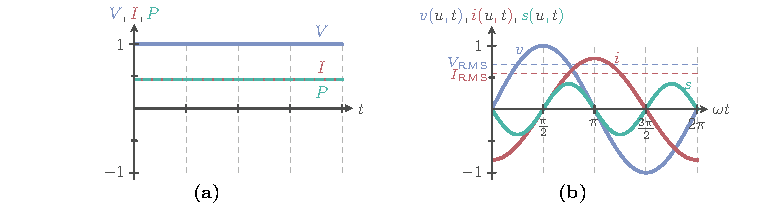
\includegraphics{foundations/figures/ac-vs-dc.pdf}
    % 
    \caption[Difference between the~\gls{ac} and~\gls{dc} model]{The
        plots for~\gls{ac} and~\gls{dc} models differ in their
        \screentextcolor{COMPLEXPOWER}{power}, \screentextcolor{CURRENT}
        {current} and
        \screentextcolor{VOLTAGE}{voltage} curves. (a) The curves of the
        linearized~\acrshort{ac} model can be interpreted like the curves of
        the~\gls{dc} model as constant functions over time. Thus,
        % 
        \screentextcolor{COMPLEXPOWER}{power~$P$}, 
        % 
        \screentextcolor{CURRENT}{current~$I$},
        % 
        and \screentextcolor{VOLTAGE}{voltage~$V$} 
        % 
        are time-independent functions. 
        (b) The~\gls{ac} model consists of sinusoid functions. The 
        % 
        \screentextcolor{COMPLEXPOWER}{instantaneous power~$
        \glssymbol{complexpower}(
        \screentextcolor{TIMESTAMP}{\vertexa}, \screentextcolor{TIMESTAMP}
        {\glssymbol{timestamp}})$},
        % 
        \screentextcolor{CURRENT}{current~$\glssymbol{current}(
        \screentextcolor{TIMESTAMP}{\vertexa}, \screentextcolor{TIMESTAMP}
        {\glssymbol{timestamp}})$},
        and
        % 
        \screentextcolor{VOLTAGE}{voltage~$\glssymbol{voltage}(
        \screentextcolor{TIMESTAMP}{\vertexa}, \screentextcolor{TIMESTAMP}
        {\glssymbol{timestamp}})$} are functions over time. The~\acrlong{rms} (\gls{rms})
        of voltage~\glssymbol{voltagerms} and current~\glssymbol{currentrms} are
        represented by the dashed-colored horizontal lines.}
    % 
    \label{ch:foundations:sec:power-flow-analyses:fig:ac-vs-dc-plots}
\end{figure}
% 
Historically, the question of whether~\gls{ac} or~\gls{dc} would be used arose
in the 1800s. There was a competition between two companies of Thomas Edison and
George Westinghouse that developed and spread the use of~\gls{dc} and~\gls{ac},
respectively. This competition is also known as \textquote{war of the currents}.
In the end~\gls{ac} imposed, since the first transformers were invented
for~\gls{ac}, allowing a simple change in voltage level and long distance
transmission as well as usage of electricity in households. The first long
distance transmission of three-phase~\gls{ac} was in 1891. It is impressive that
the first pure~\gls{dc} transformer was invented in 1976, since technologies
such as semiconductors had been developed. Nowadays, the question arises in
terms of distribution systems~\parencite{Ham07}.

However, if we look at the current power grid, we mainly have an~\gls{ac} power
grid with a few~\gls{hvdc} lines. So we focus on the question of whether our
model assumptions are reasonable and when the errors would become significant.
Recall that the~\gls{dc} power flow model introduces three assumptions (\gls{dc}
Assumptions~\ref{ch:foundations:sec:power-flow-analyses:assumption:negligible-resistance}--\ref{ch:foundations:sec:power-flow-analyses:assumption:voltage-magnitude})
that simplify the~\gls{ac} power flow to a~\gls{dc} power flow model. The
question of when the~\gls{dc} model is useful, thus, depends on three
parameters: resistance of the lines, voltage angle differences, and voltage
magnitude deviations. An evaluation that tests the three assumptions is given
by~\textcite{Pur05}.

The~\gls{tso}{s} usually say that the resistance of the transmission network is
negligible. This statement is basically covered
in~$\cref{ch:foundations:sec:power-flow-analyses:assumption:negligible-resistance}$.
The transmission network in Germany has voltages of 110~\gls{kv}, 220~\gls{kv},
and 380~\gls{kv}. These voltage layers define the high voltage level. The higher
the voltage the lower the current and thus, the lower the influence of the
resistance
(see~\cref{ch:foundations:sec:power-flow-analyses:eq:complex-power-flow:pqv:rectangular:2,ch:foundations:sec:power-flow-analyses:eq:dc:ohms-law:1}).
So our expectation would be that this assumption mainly depends on the voltage
level and on the line resistances. \textcite[p.4]{Pur05} show that for the
Belgian grid with voltage levels of~$70$~\gls{kv}, $150$~\gls{kv},
$220$~\gls{kv}, and~$380$~\gls{kv} the~$\nicefrac{\reactances}{\resistances}$
ratio ranges from~$0.8$ for the~$70$~\gls{kv} voltage level to~$12.5$ for
the~$380$~\gls{kv} voltage level. The real power estimation error (that
increases with increasing resistance) for these voltage levels is less
than~$5\%$ and for the~$380~\gls{kv}$ power grid drops below~$2.5\%$. Both
errors are small and thus, the resistance for
such~$\nicefrac{\reactances}{\resistances}$ ratios in high voltage levels is
negligible.% This particularly means that for high-voltage levels the resistance is
% the main factor.\franzi{Was wollte ich damit sagen???}

The~\cref{ch:foundations:sec:power-flow-analyses:assumption:voltage-angle-difference}
assumes that the voltage angle difference is small enough such that the sine
function is negligible. The system's stability is guaranteed in the range of~$
[-\nicefrac{\gls{pi}}{2};\nicefrac{\gls{pi}}{2}]$. However, $30^\circ$ or~$[ -
\nicefrac{\gls{pi}}{6};\nicefrac{\gls{pi}}{6} ]$ is the range where the sine can be
approximated by~$\sin(x) = x$. Thus, if the difference is within this range, the
real power error should be small. \textcite[p.2]{Pur05} evaluate for the Belgian
power grid with voltages ranging from~$70$~\gls{kv} to~$380$~\gls{kv} that the
highest voltage angle difference was~$7^\circ$ and in~$94\%$ of the lines it was
less than~$2^\circ$. One explanation is that the inductive and conductive
properties of an edge are quite small. However, the lines inductive property is
usually slightly higher, though for long distances the capacitive property
increases (see the transmission line representation section
in~\cref{ch:foundations:sec:power-flow-analyses:subsec:AC-Model} on
Page~\pageref{ch:foundations:sec:power-flow-analyses:transmission-line-representation}).

The last
assumption---\cref{ch:foundations:sec:power-flow-analyses:assumption:voltage-magnitude}\!\!---is
about a flat voltage profile, \eg, all voltages are equal to~$1$~\glssymbol{pu}.
If there is a voltage deviation then this would automatically lead to a voltage
difference that is simply not modeled in the~\gls{dc} model. The real power
error increases with increasing voltage deviation~\parencite[p.4; Figure
7]{Pur05}. Thus, a flat voltage profile is important but difficult to establish
in power grids.  %\franzi{flat voltage profile means that the standard deviation
% < 0.01}

This particularly means that the most critical assumption is the flat voltage
profile. The others can be at least established quite well in a high voltage
power grid. However, flat voltage profiles are difficult to establish and thus,
the results have to be carefully interpreted in terms of an~\gls{ac} power
grid. However, this discussion also shows that the more complex Sin-model
including the sine function might be a more realistic model, but that the
assumption is not critical for the real power error and thus, it might increase
the complexity unnecessarily. However, from a theoretical perspective this
model is quite interesting as the feasibility problem is already strongly
\NP-hard~\textcite{Bie19}.
% 
%%%%%%%%%%%%%%%%%%%%%%%%%%%%%%%%%%%%%%%%%%%%%%%%%%%%%%%%%%%%%%%%%%%%%%%%%%%%%%%%
\paragraph{Problems}%
\label{ch:foundations:sec:power-flow-analyses:problems}%
%%%%%%%%%%%%%%%%%%%%%%%%%%%%%%%%%%%%%%%%%%%%%%%%%%%%%%%%%%%%%%%%%%%%%%%%%%%%%%%%
% 
The~\gls{ac} feasibility problem is a subproblem of many
optimization problems such as the~\acrlong{tnep} (\gls{tnep}) problem, 
the~\acrlong{otsp} (\gls{otsp}) and
the~\acrlong{mpfp} (\gls{mpfp}).

% the~\acrlong{edp} (\gls{edp}), the~\acrlong{ucp} (\gls{ucp})
The~\acrlong{edp} (\gls{edp}) minimizes the total cost represented by the sum of
all generator cost functions~\cost. It is the simplest problem formulation that
checks whether demand and supply match by abstracting from the power grid and
incorporates the energy balance equation, and the generator constraints
(see~\cref{ch:foundations:sec:power-flow-analyses:eq:network:bounds:real-power-injection,ch:foundations:sec:power-flow-analyses:eq:network:bounds:reactive-power-injection}).
After adding the power grid specifics, the problem is called either~\gls{ac}
or~\gls{dc}~\acrlong{opfp} (\gls{opfp}). All the problems mentioned so far have
continuous variables only.
% 
In terms of planning problems, we introduce integer or binary variables. The
most commonly known problems for finding an optimal topology are~\gls{tnep},
\gls{otsp}, and \gls{mtsfp}.
%  
% % 
% %%%%%%%%%%%%%%%%%%%%%%%%%%%%%%%%%%%%%%%%%%%%%%%%%%%%%%%%%%%%%%%%%%%%%%%%%%%%%%%%
% \section{Experimental Setup}\label{ch:foundations:sec:experimental-setup}
% %%%%%%%%%%%%%%%%%%%%%%%%%%%%%%%%%%%%%%%%%%%%%%%%%%%%%%%%%%%%%%%%%%%%%%%%%%%%%%%%  

% \paragraph{Methodology} TODO
% -c++
% -gcc and flags


% \paragraph{Benchmark Data} TODO
% - Table about the Instance, Electrical network, Number of Vertices and number of
% edges


% % 
% \begin{table}[t!]
%     \centering
%     \input{foundations/tables/tbl-benchmarkCases-powerGrid.tex}
%     % 
%     \caption{
%     Overview of the~\gls{ieee} instances used in this work. The table shows the
%     instance name, the power grid it represents, the number of vertices~$
%     \fmagnitude{\glssymbol{vertices}}$, the number of edges~$\fmagnitude{\glssymbol{edges}}$, the
%     number of generators~$\fmagnitude{\generators}$, and the number of~$
%     \fmagnitude{\consumers}$.
%     % 
%     }
%     % 
%     \label{ch:foundations:tbl:load-flow-bus-specification}
% \end{table}

% \paragraph{Implementation Details} TODO